% !TEX root = ../../main.tex

\subsection{Characterisation of trends}\label{def:trends}

The graphs in \autoref{def:fgr:tga-defects} summarize the 
trends in missing linker defects as calculated through 
the TGA plateau at \SI{420}{\degreeCelsius}. The DMF leached samples,
due to the multiple datapoints with different acid concentrations
show the clearest influence of this variable on defect
generation. Even small amounts of modulator leads to the decrease of 
the linker-to-node ratio, but the increase in concentration stops 
having an effect at around 20:1 equivalents. It is likely that
the trends are similar with other solvents, even if less 
datapoints are available.

\begin{figure}[htb]
    \centering

    \begin{subfigure}{0.25\linewidth}
        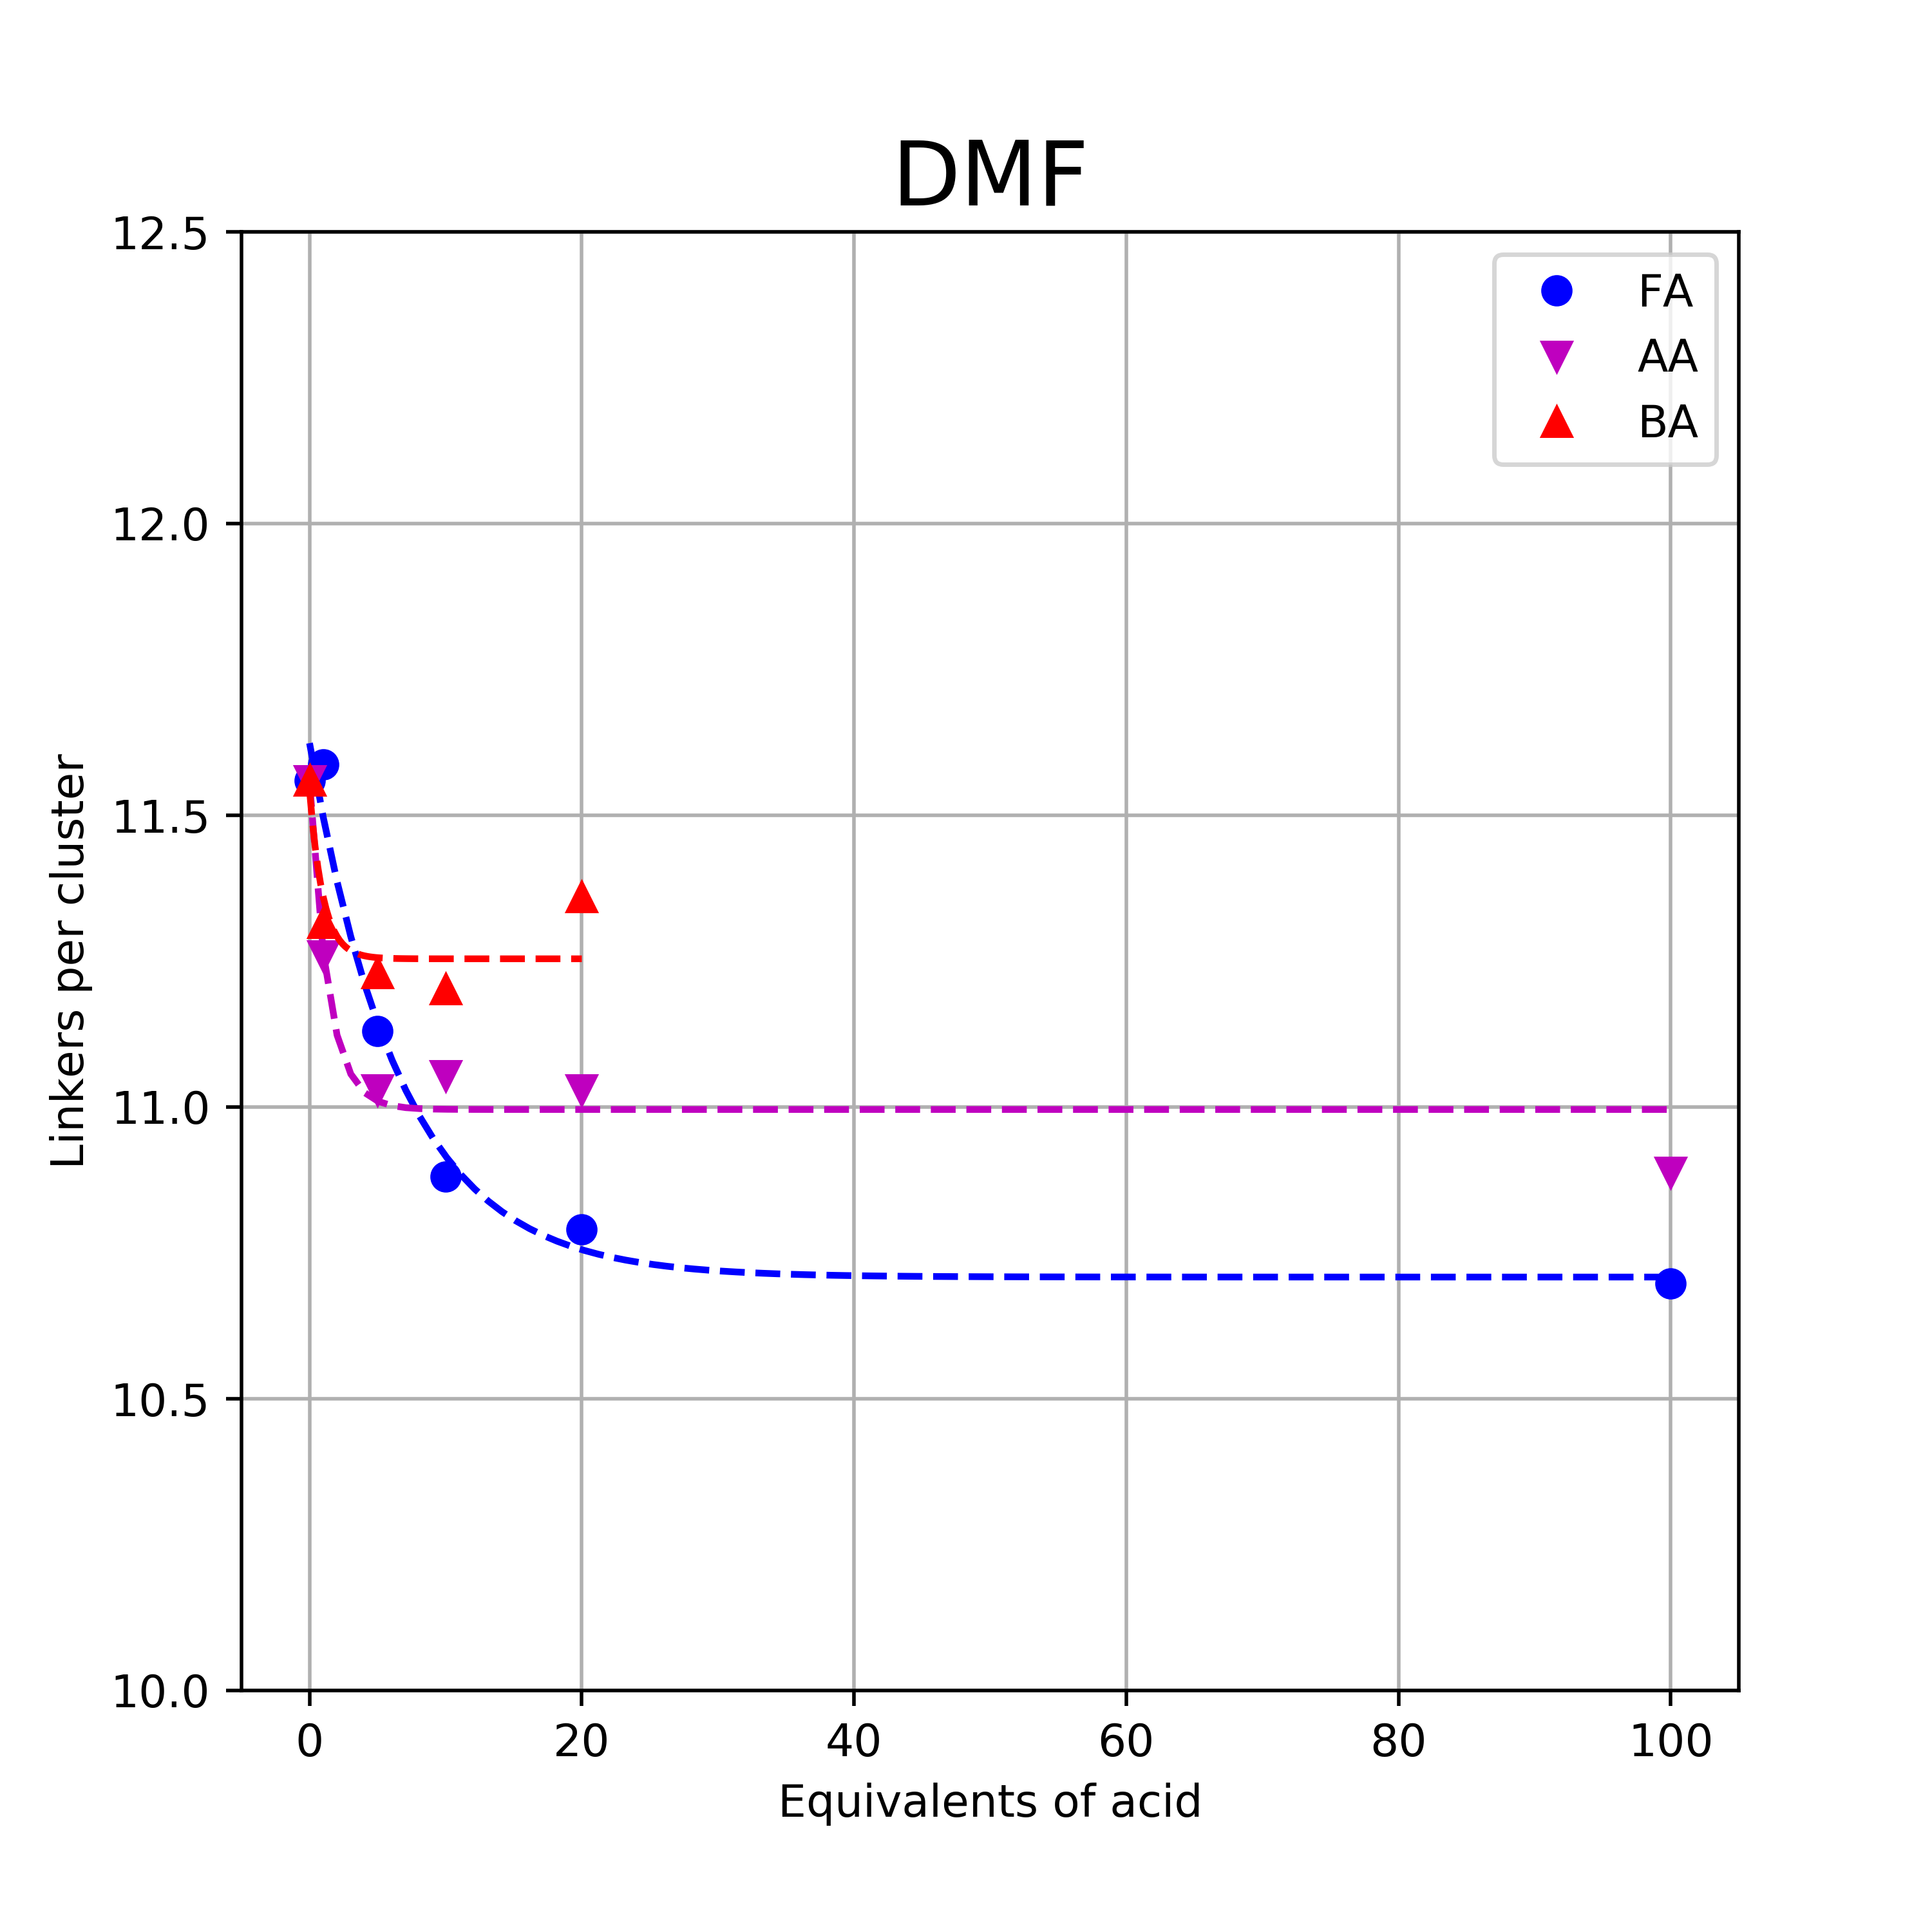
\includegraphics[width=\textwidth]{tga/DMF-def-overview}%
        \caption{}%
        \label{def:fgr:tga-dmf-linkers}
    \end{subfigure}%
    \begin{subfigure}{0.25\linewidth}
        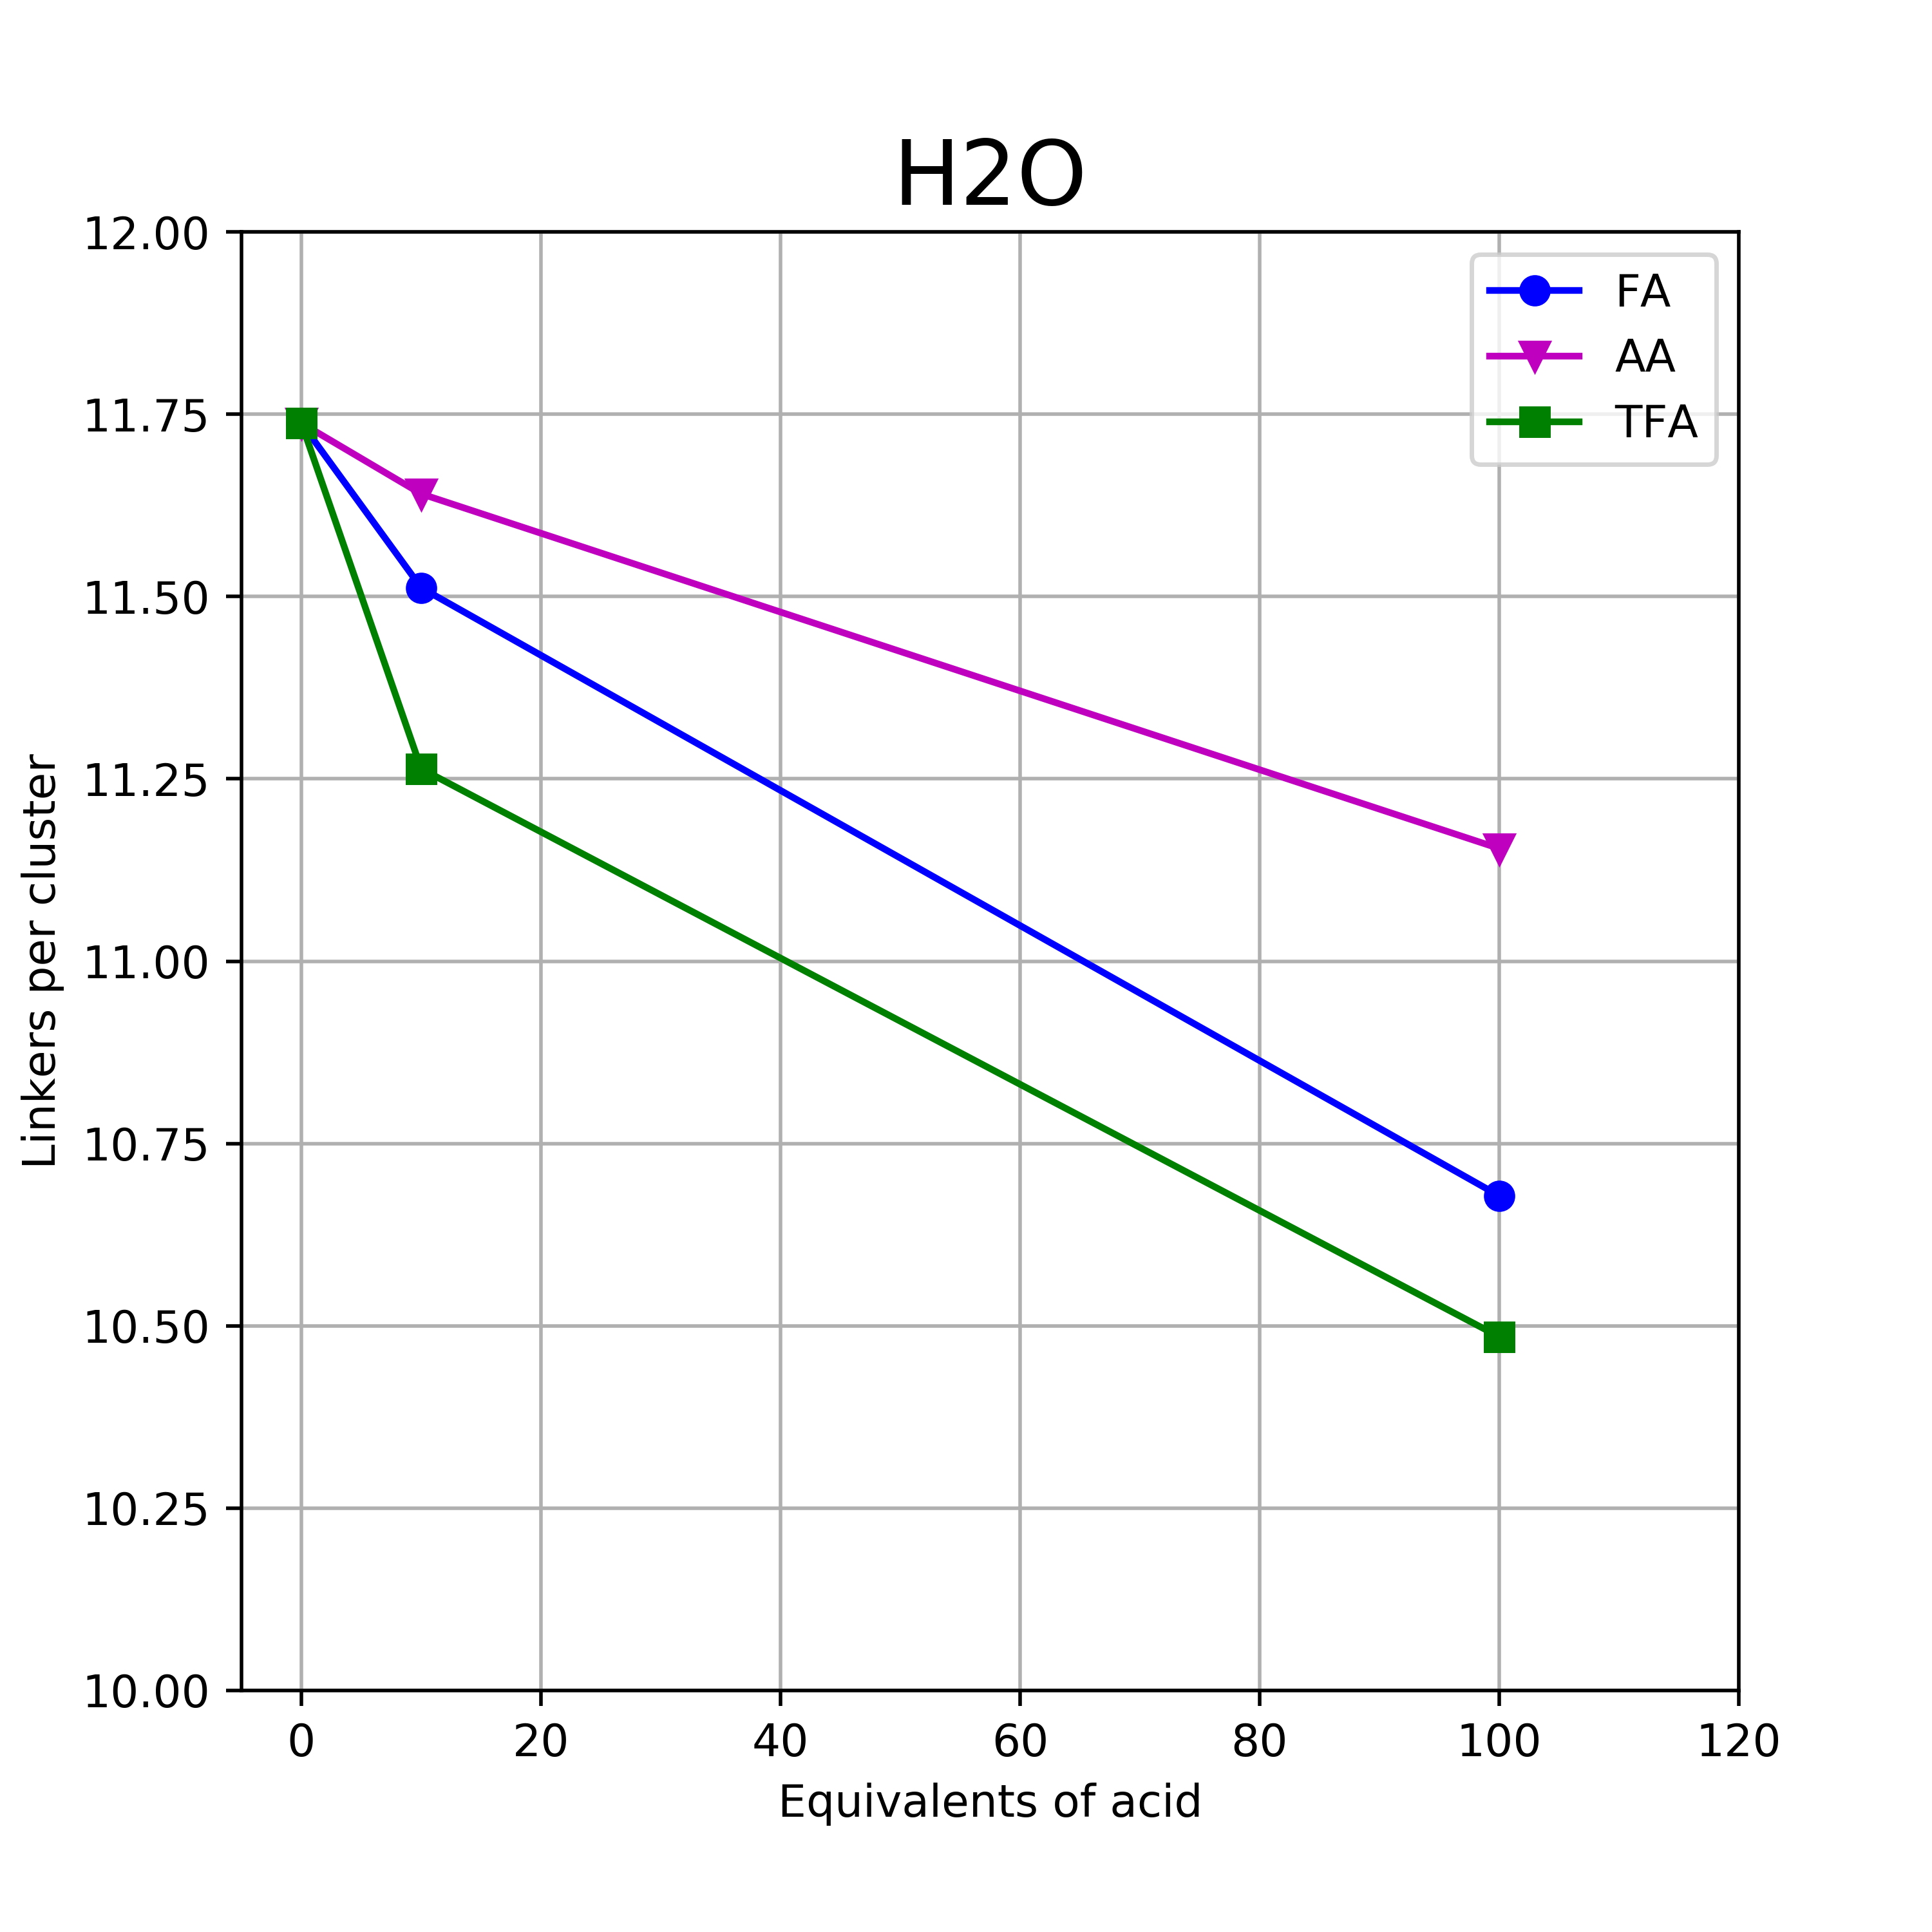
\includegraphics[width=\textwidth]{tga/H2O-def-overview}%
        \caption{}%
        \label{def:fgr:tga-h2o-linkers}
    \end{subfigure}%
    \begin{subfigure}{0.25\linewidth}
        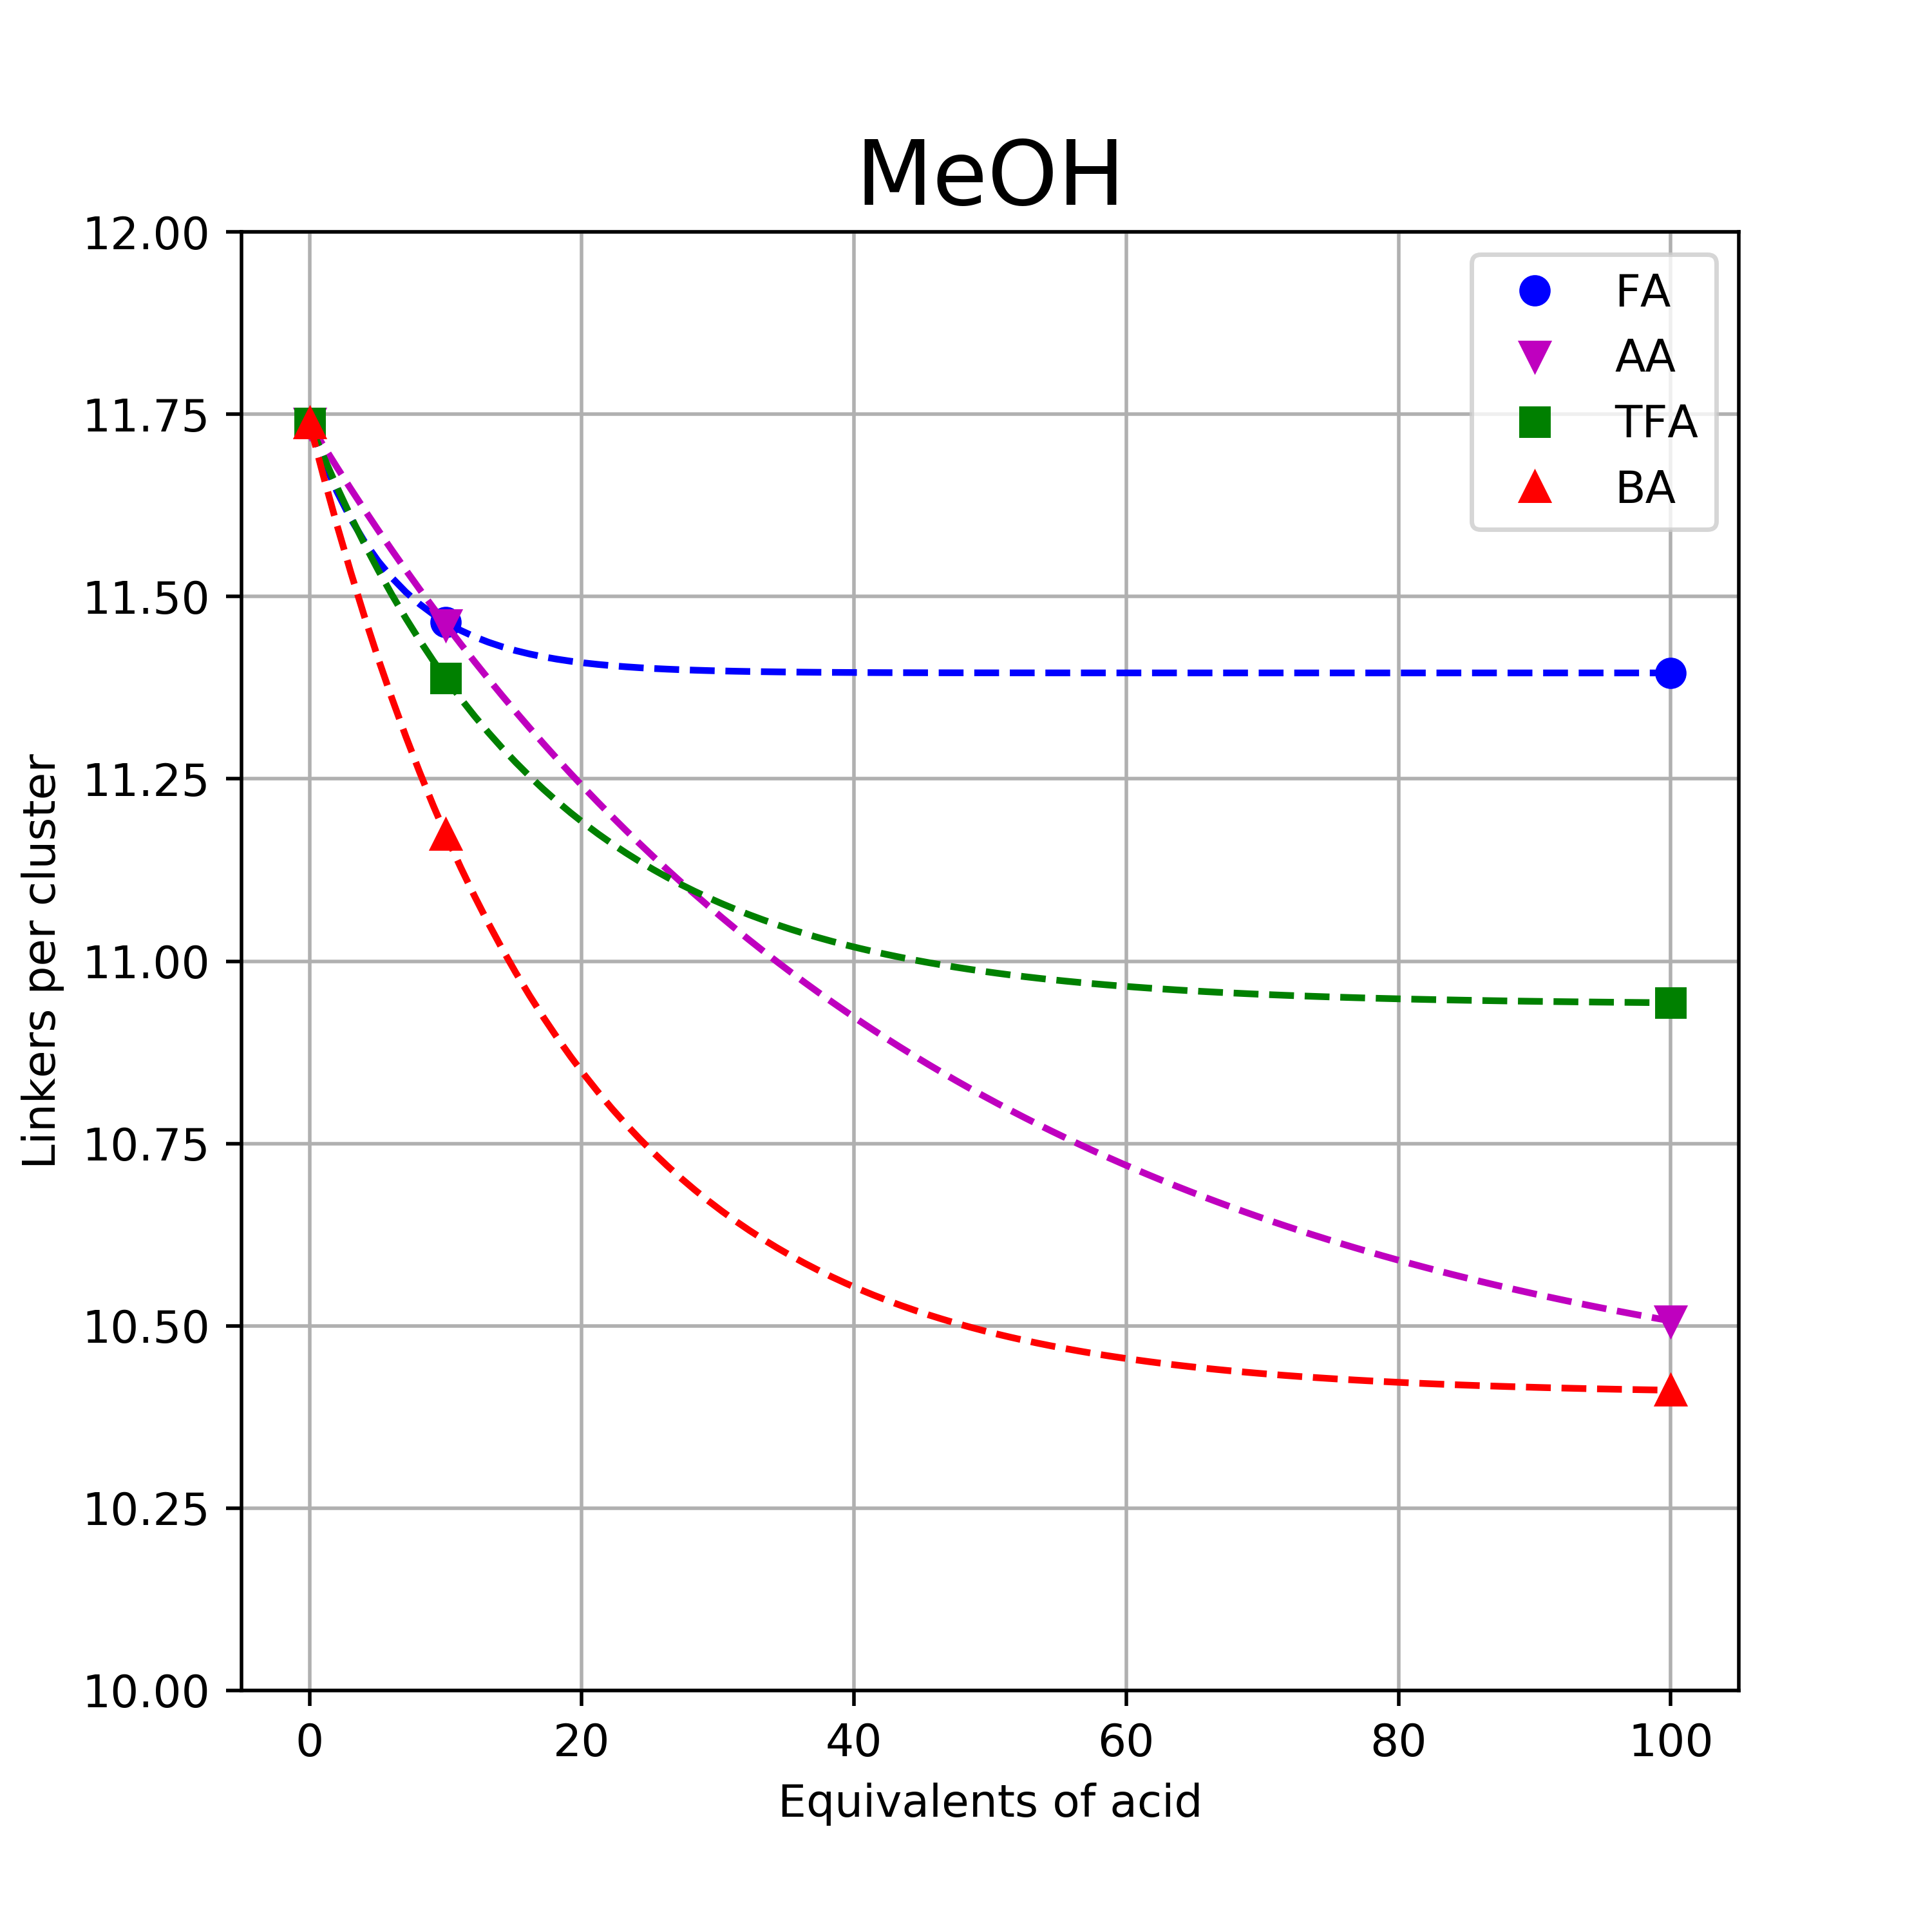
\includegraphics[width=\textwidth]{tga/MeOH-def-overview}%
        \caption{}%
        \label{def:fgr:tga-meoh-linkers}
    \end{subfigure}%
    \begin{subfigure}{0.25\linewidth}
        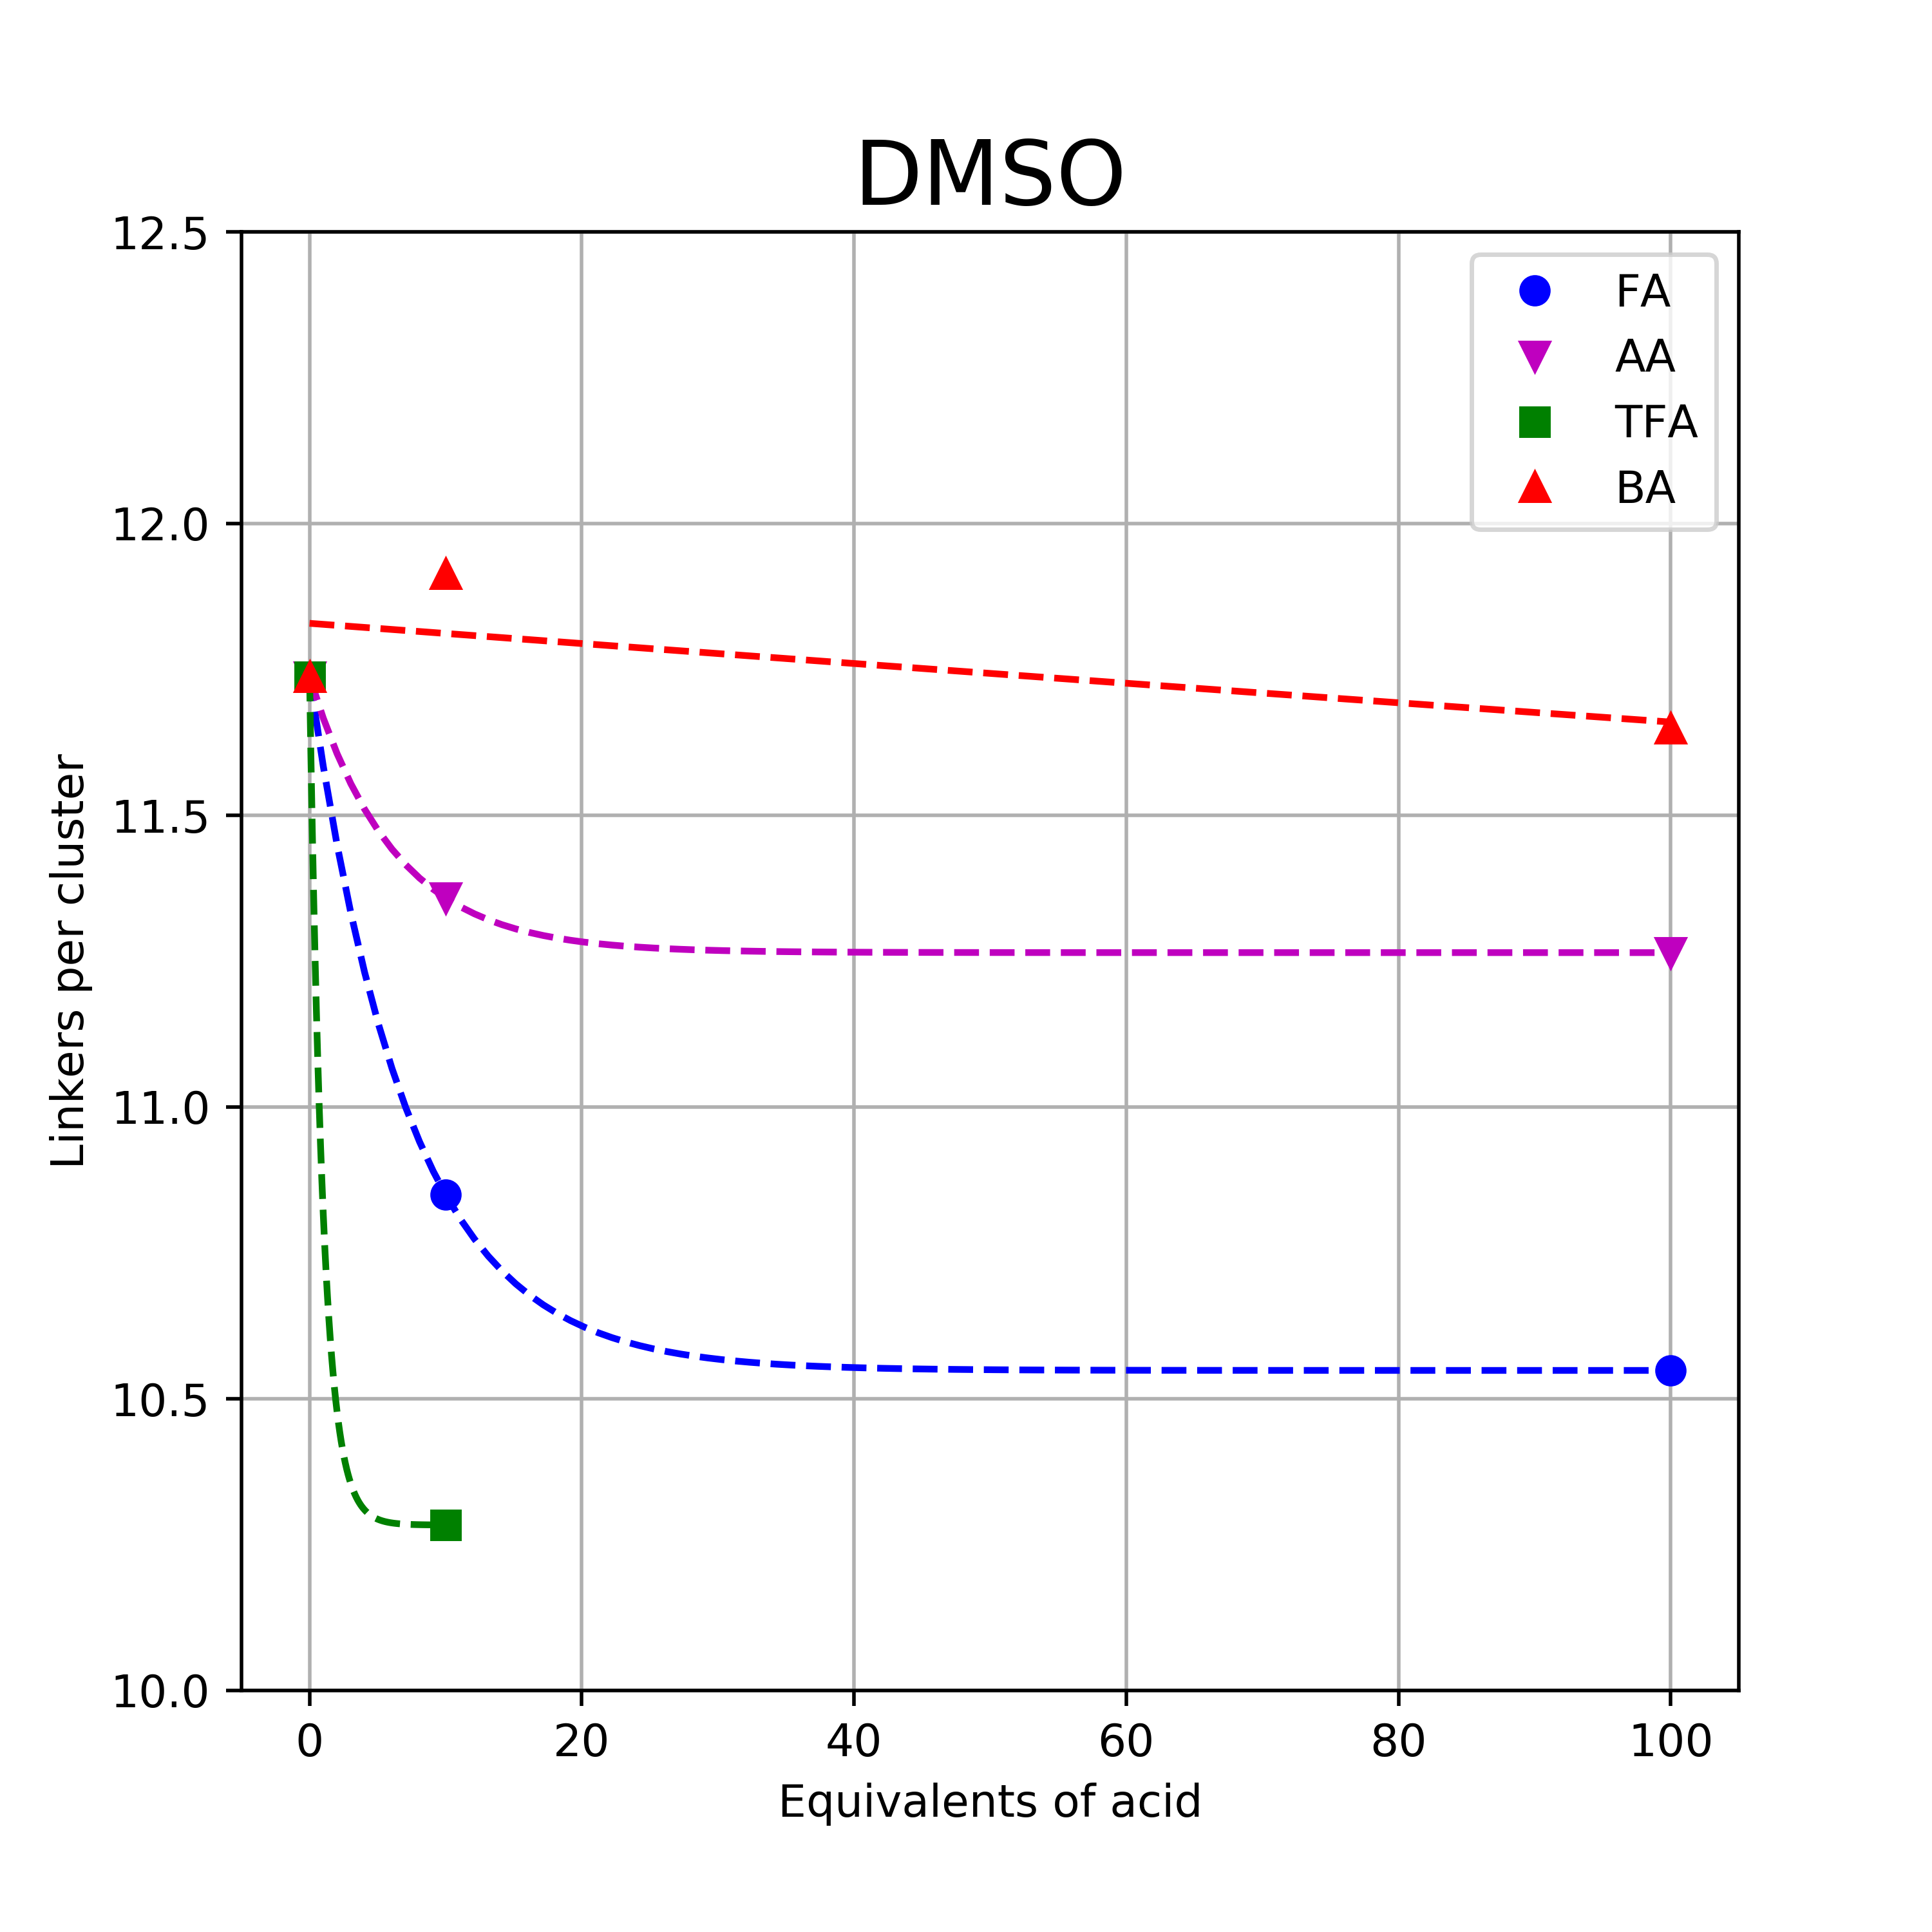
\includegraphics[width=\textwidth]{tga/DMSO-def-overview}%
        \caption{}%
        \label{def:fgr:tga-dmso-linkers}
    \end{subfigure}%

    \caption{Calculated linker-to-node ratio from the TGA curve 
    normalized mass at \SI{420}{\degreeCelsius} for (a) DMF 
    (b) \ce{H2O}, (c) \ce{MeOH} and (d) DMSO leached samples.
    A ratio of 12 to 1 corresponds to a completely defect-free
    structure. An exponential decay trendline is fitted to 
    each set of points.}%
    \label{def:fgr:tga-defects}
    
\end{figure}

In the case of benzoic acid the data bears careful interpretation. 
Thermogravimetric methods may not be suitable 
for assessing the resulting defects. The comparatively large molecule,
high boiling point and similarity to the terephtalate linker
make the removal of benzoic acid capping open metal sites harder, and
as such, the plateau is not an accurate indication of defectivity.
Indeed, the calculated linker ratio is seen to actually increase in 
the case of methanol and DMSO. We propose that in benzoic acid 
leached samples defect generation occurs through the coordination
of two benzoic molecules (or one, in the case of a ``dangling'' linker), 
as seen in \autoref{def:fgr:benzoic-defect},
with the increased amount of organic material effectively compensating
for any defects that could be seen in the TGA curve.

\begin{figure}[htb]
    \centering
    \( \vcenter{\hbox{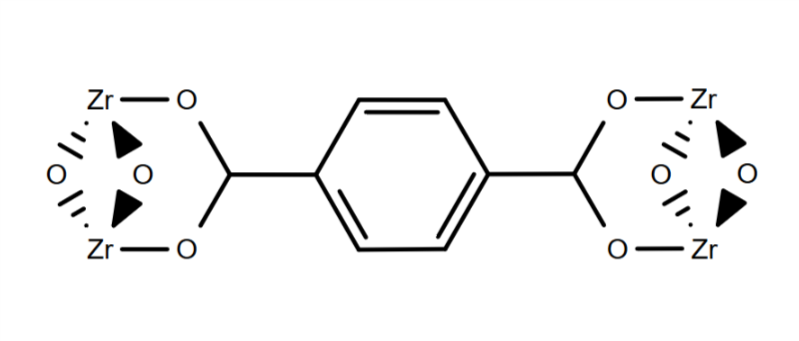
\includegraphics[width=0.3\linewidth]{structures/site-linker}}}\)%
    \( \longrightarrow \)%
    \(\vcenter{\hbox{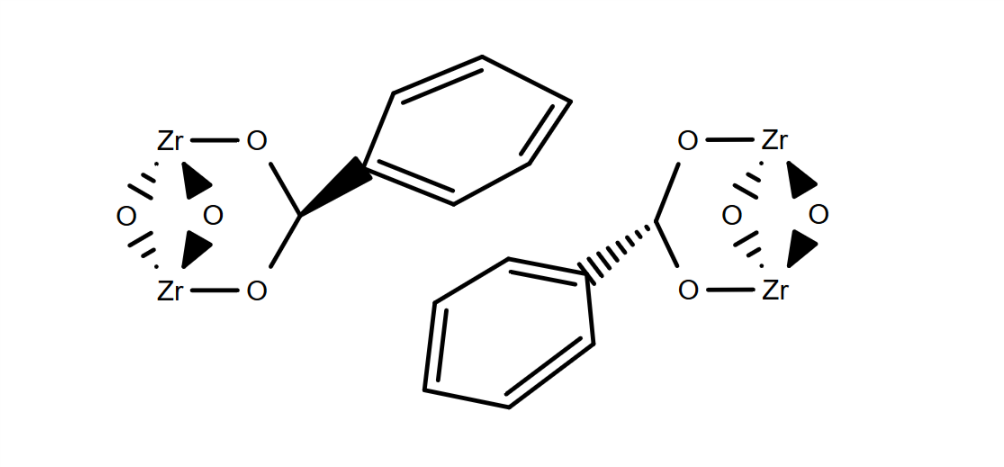
\includegraphics[width=0.4\linewidth]{structures/site-benzoic}}}\)
    \caption{A defect site created through benzoic acid.}%
    \label{def:fgr:benzoic-defect}
\end{figure}

For the nitrogen adsorption dataset, the predictors described in the 
previous section have been calculated using the pyGAPS framework
(methods are described in \autoref{pyg}). The Henry constant is determined 
through the initial slope method, with a linear section found below 
\(10^{-4}~p/p_0\). Total pore volume is taken as the liquid density
of the amount adsorbed at \(0.8~p/p_0\), assuming that 
nitrogen is in a liquid-like state in the MOF pores. The pore
size distribution was calculated through the Horvatz-Kawazoe
method for micropores, the Dollimore-Heal method for mesopores
and DFT kernel fitting for a multiscale distribution. While 
the applicability of these methods for determination of absolute
pore size of the UiO-66 framework may be put into question, 
they can be readily used to compare between different samples
of the same material.
In general, the leaching process has a positive effect on 
surface area and pore volume, both of which increase 
with a higher concentration of acid used. The strength of 
the initial interaction of the nitrogen probe with the pore 
walls is changed as well, with more defective samples likely
to have a more pronounced interaction, either through the introduction
of CUS or modification of pore environment.

\begin{figure}[htb]
    \centering

    \begin{subfigure}{0.25\linewidth}
        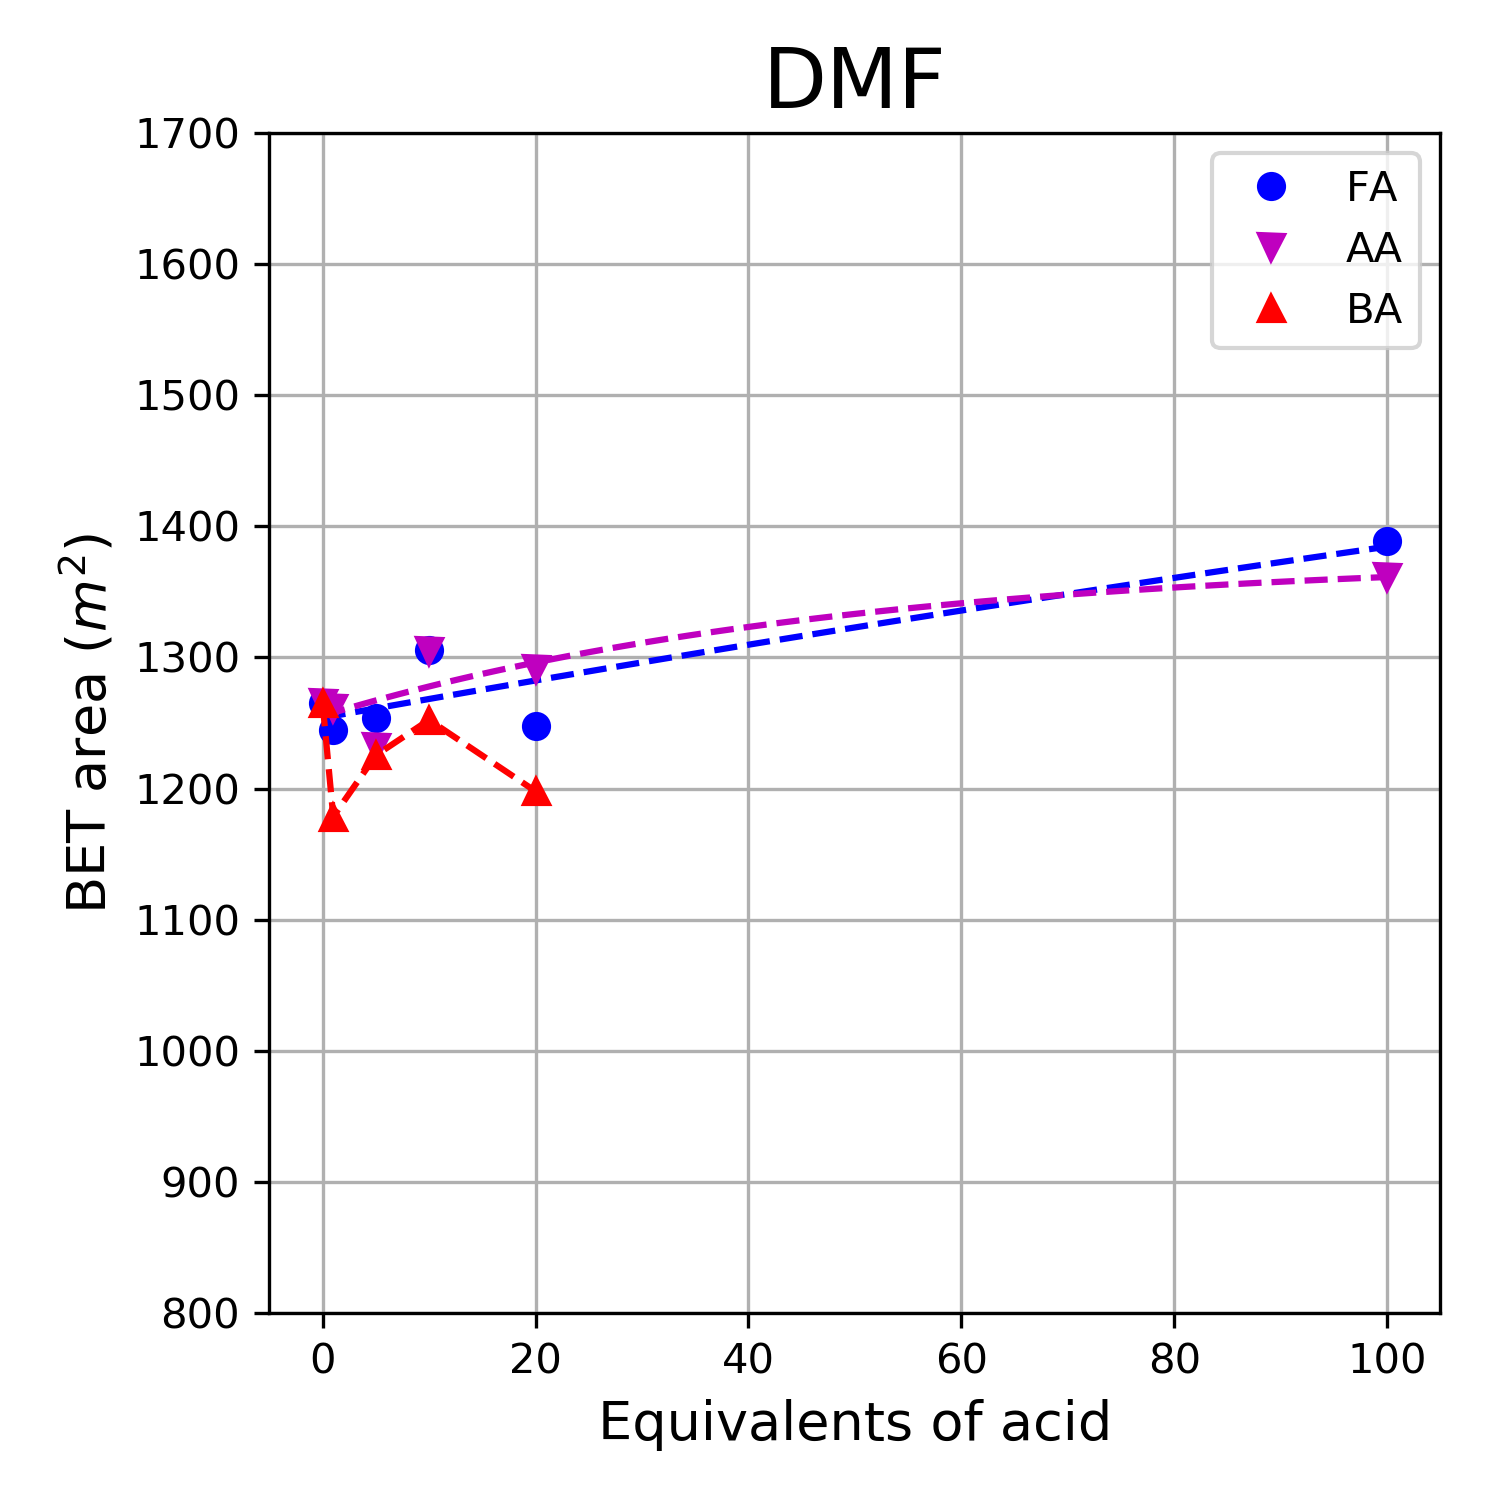
\includegraphics[width=\textwidth]{n2phys/dmf-area}%
        \caption{}%
        \label{def:fgr:n2phys-dmf-area}
    \end{subfigure}%
    \begin{subfigure}{0.25\linewidth}
        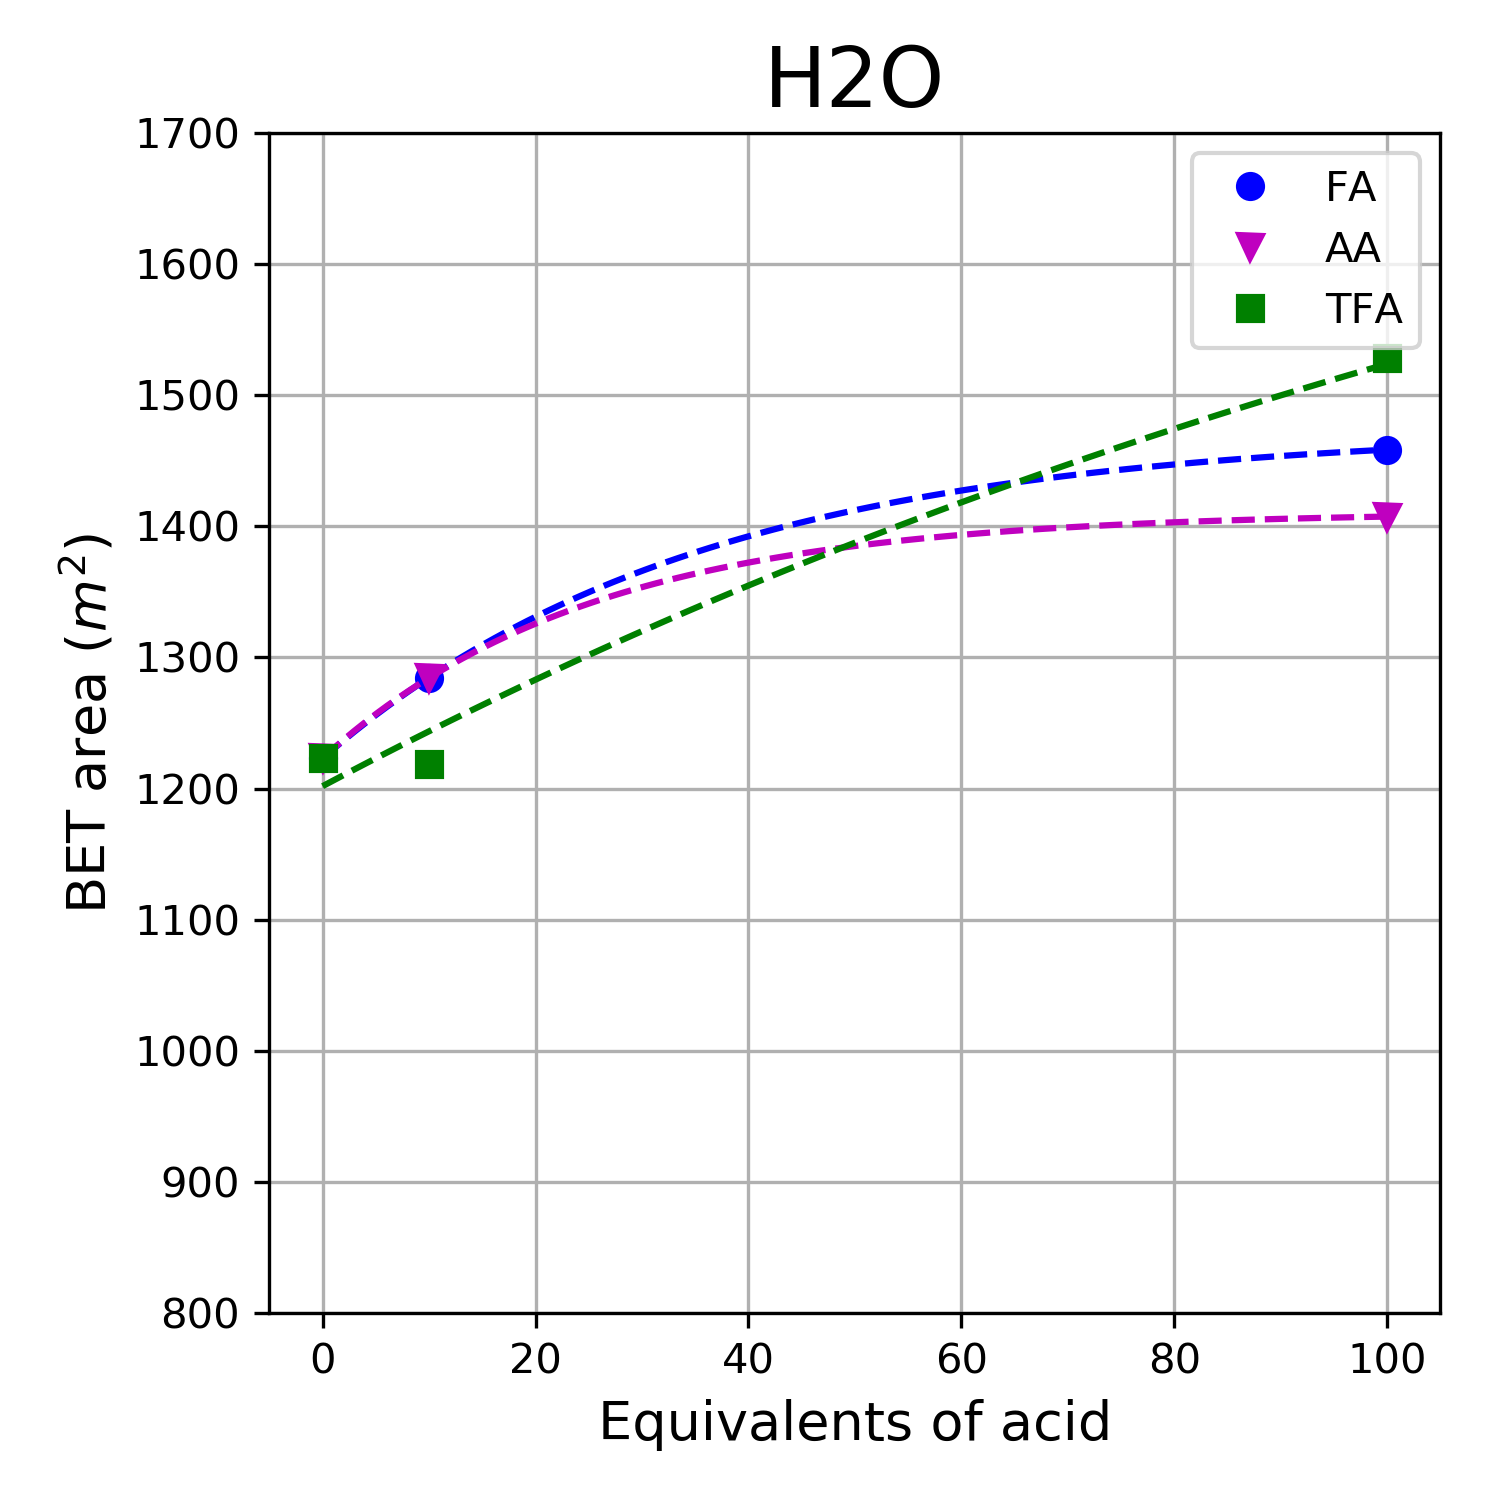
\includegraphics[width=\textwidth]{n2phys/h2o-area}%
        \caption{}%
        \label{def:fgr:n2phys-h2o-area}
    \end{subfigure}%
    \begin{subfigure}{0.25\linewidth}
        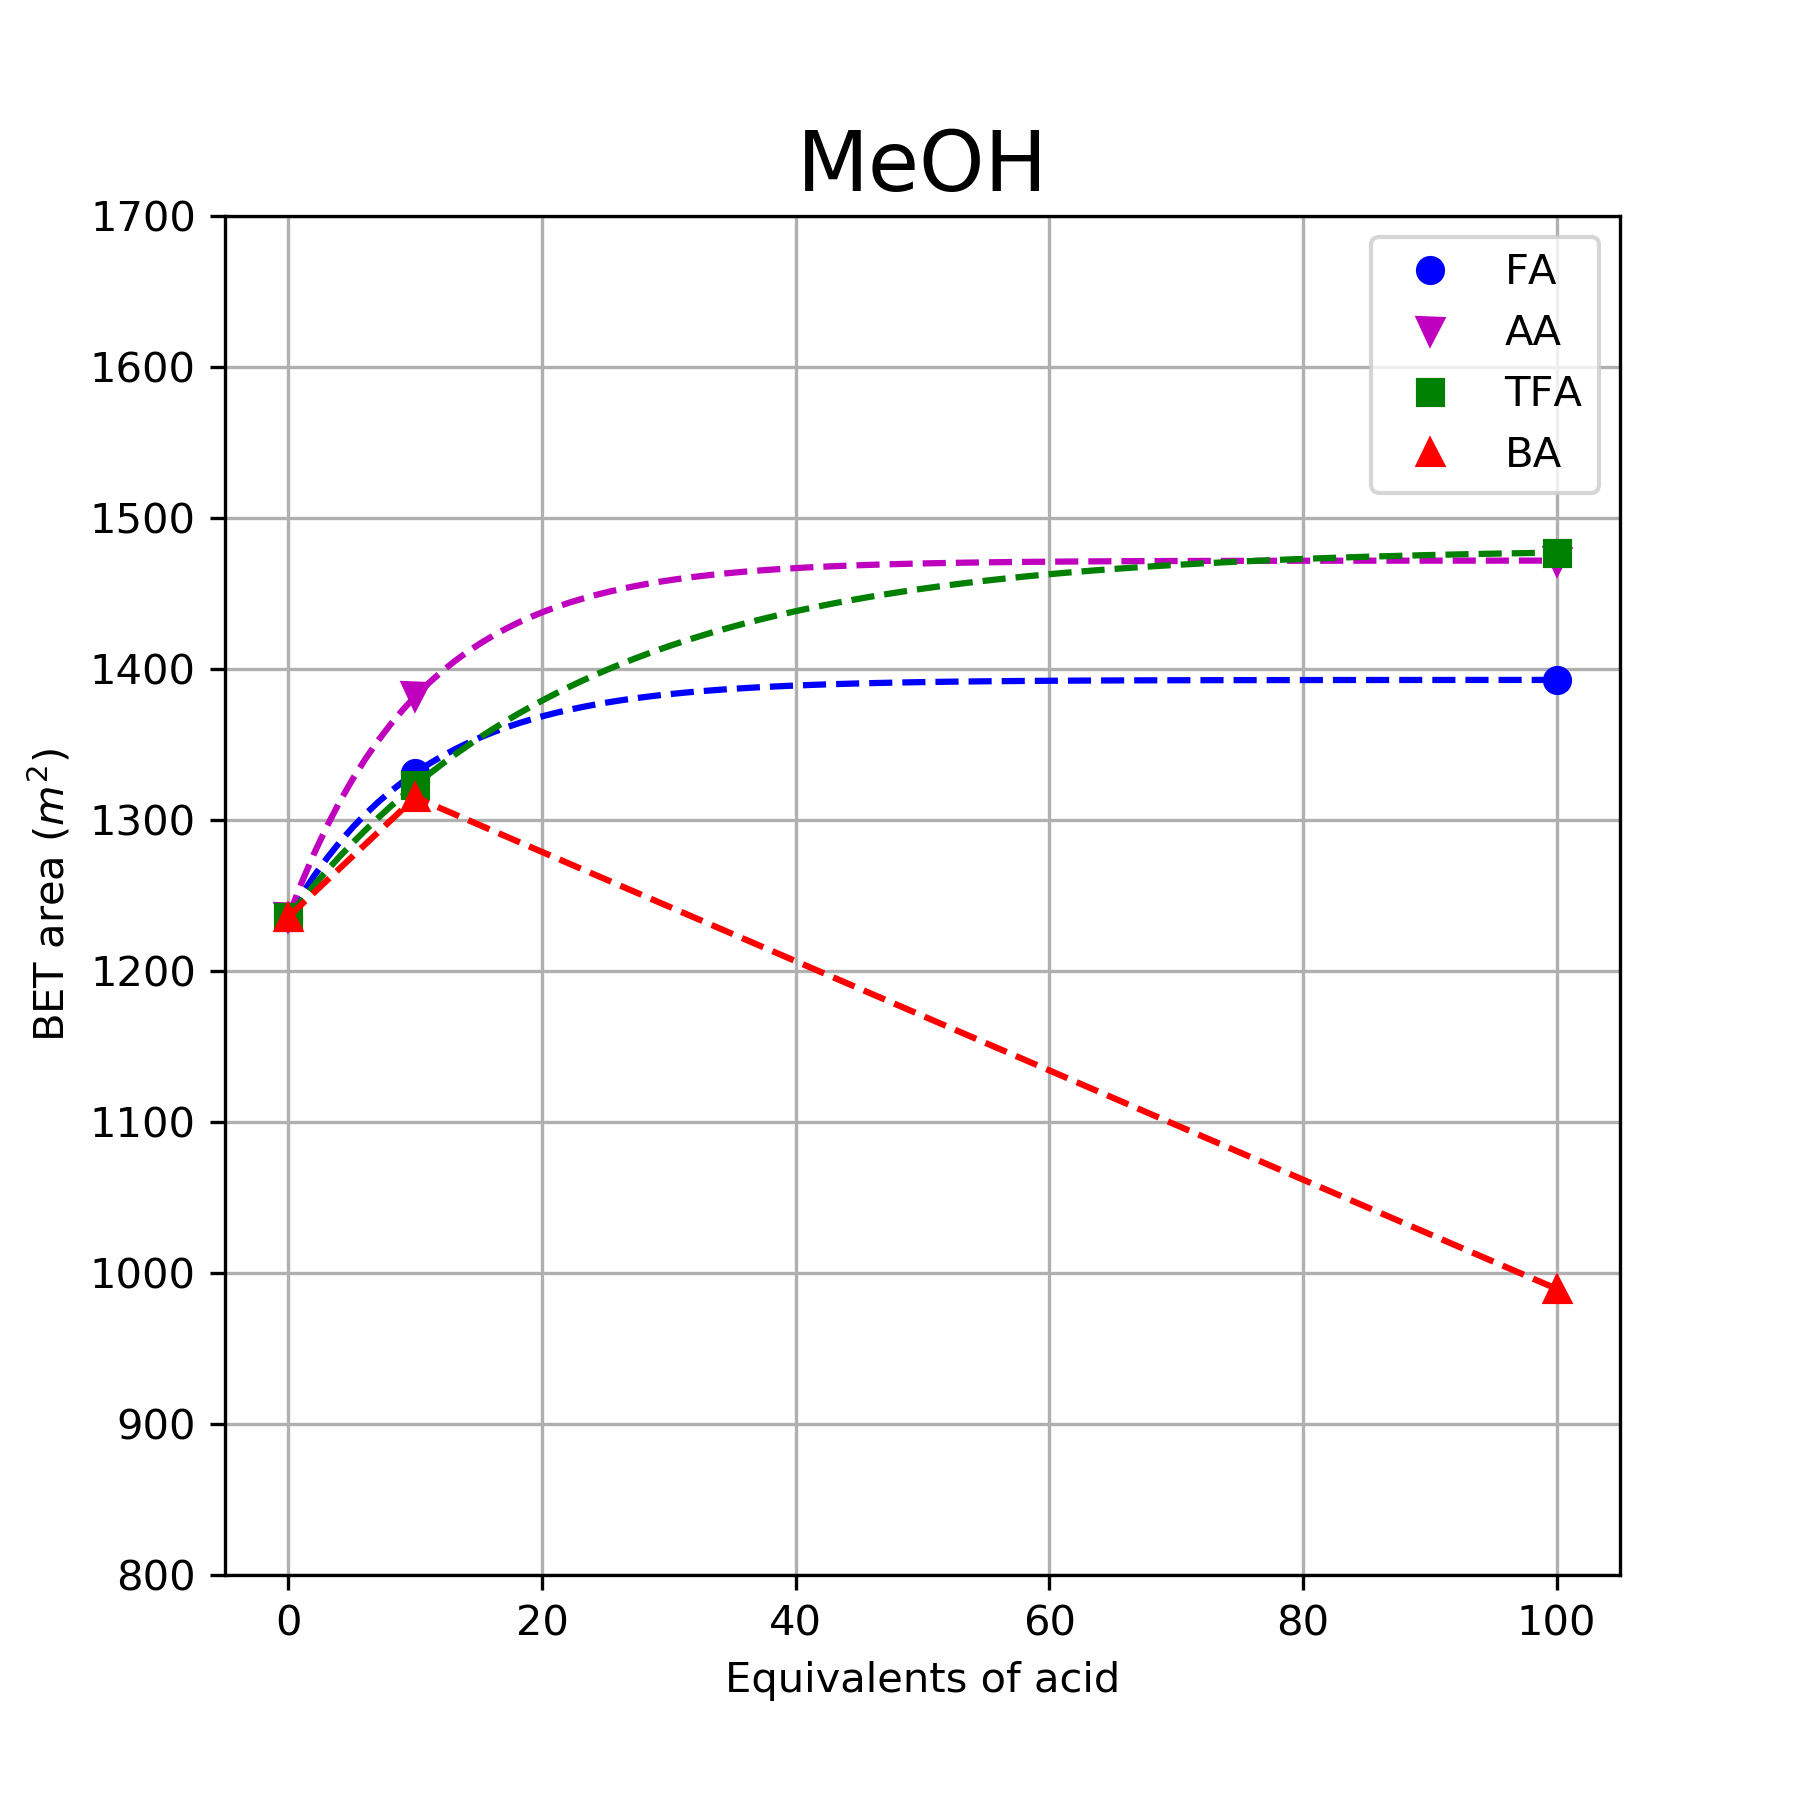
\includegraphics[width=\textwidth]{n2phys/meoh-area}%
        \caption{}%
        \label{def:fgr:n2phys-meoh-area}
    \end{subfigure}%
    \begin{subfigure}{0.25\linewidth}
        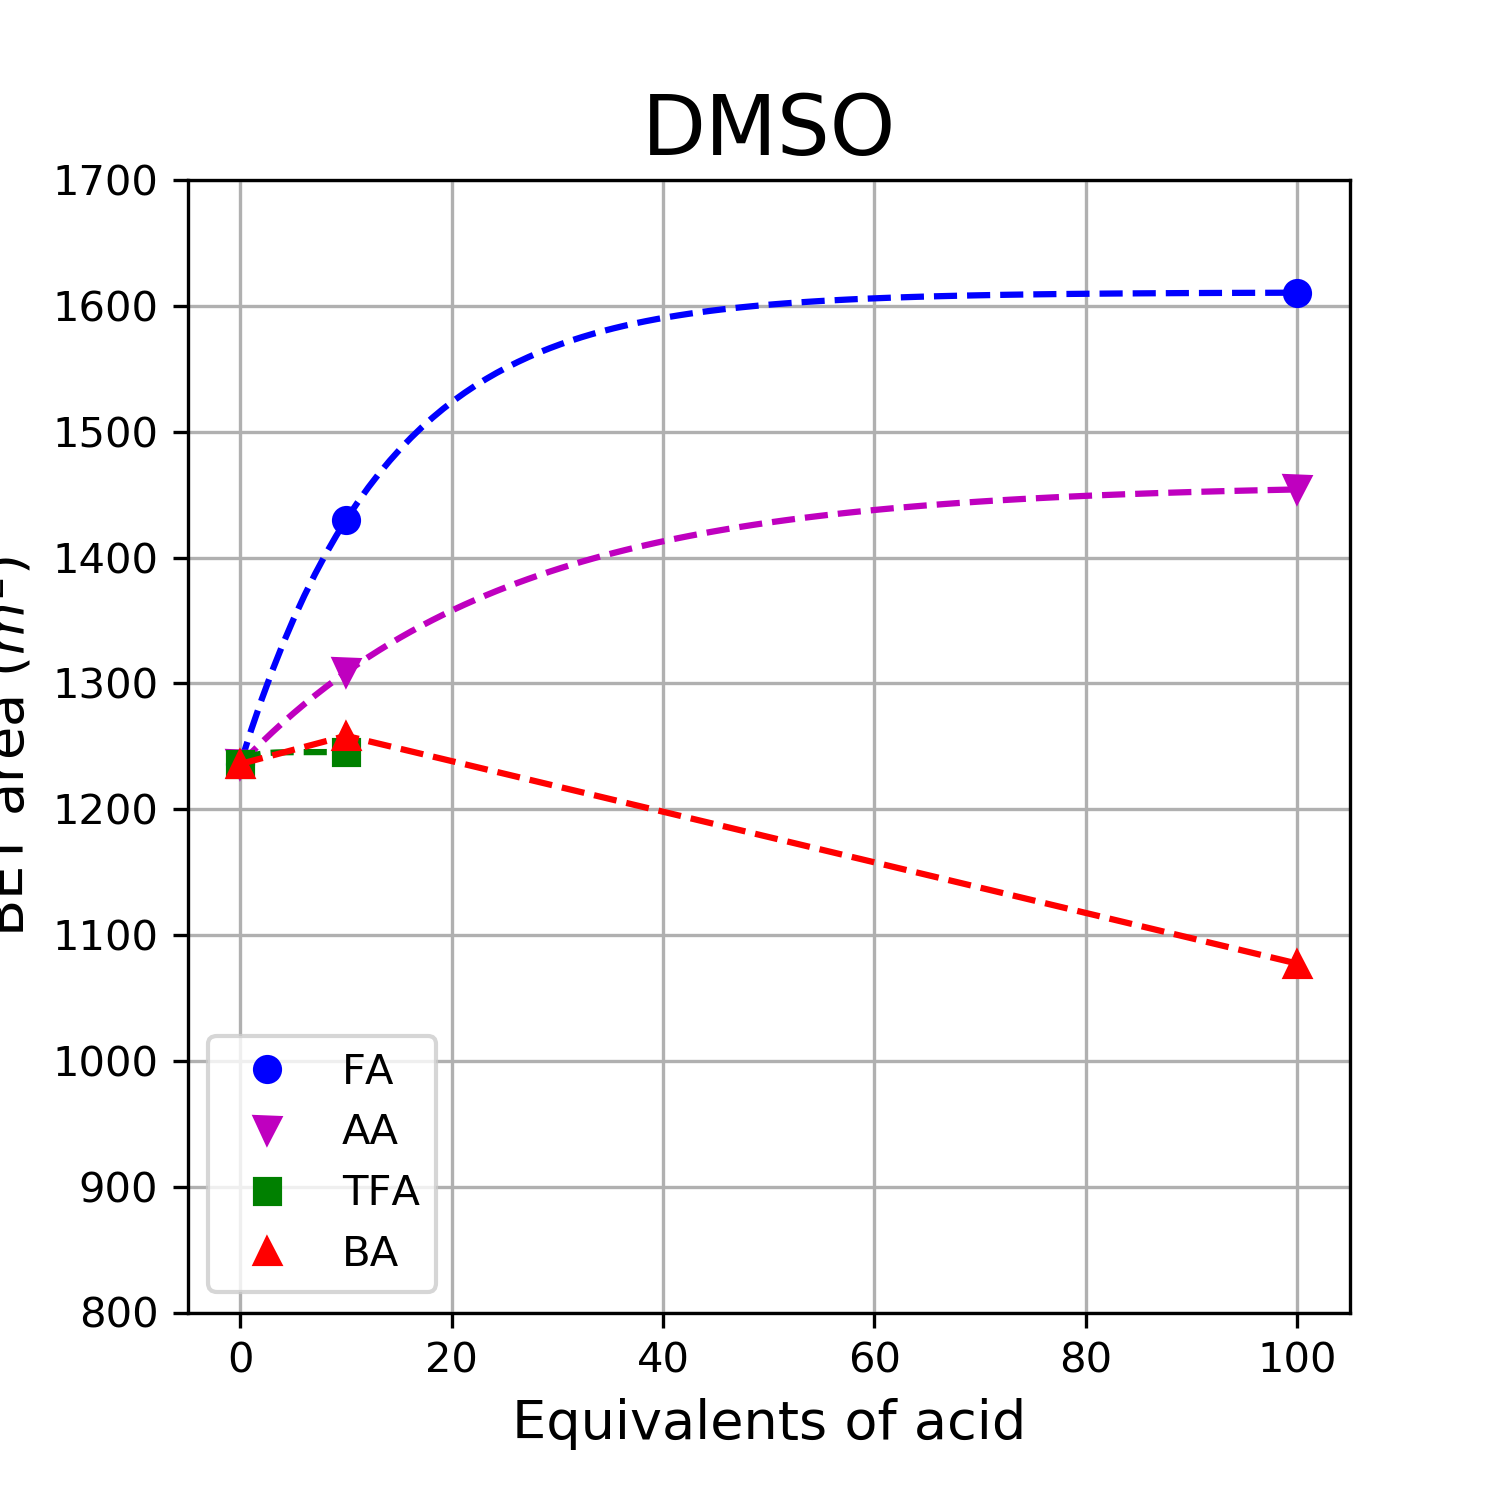
\includegraphics[width=\textwidth]{n2phys/dmso-area}%
        \caption{}%
        \label{def:fgr:n2phys-dmso-area}
    \end{subfigure}%

    \begin{subfigure}{0.25\linewidth}
        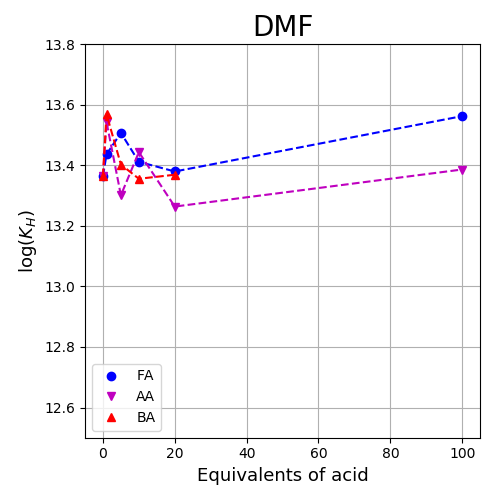
\includegraphics[width=\textwidth]{n2phys/dmf-henry}%
        \caption{}%
        \label{def:fgr:n2phys-dmf-henry}
    \end{subfigure}%
    \begin{subfigure}{0.25\linewidth}
        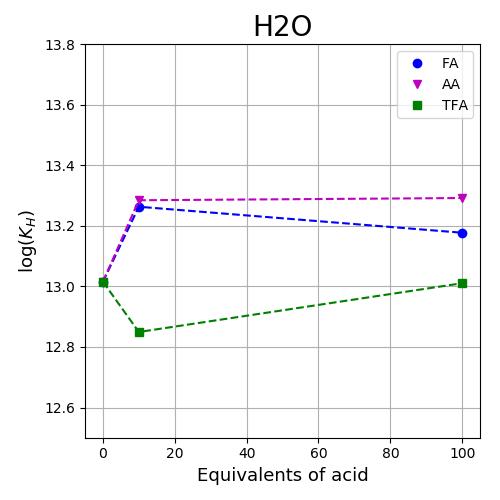
\includegraphics[width=\textwidth]{n2phys/h2o-henry}%
        \caption{}%
        \label{def:fgr:n2phys-h2o-henry}
    \end{subfigure}%
    \begin{subfigure}{0.25\linewidth}
        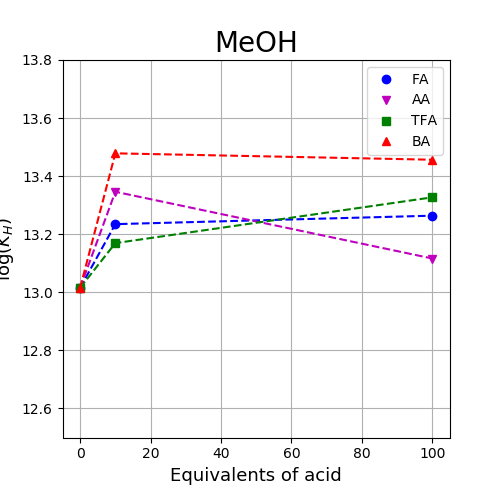
\includegraphics[width=\textwidth]{n2phys/meoh-henry}%
        \caption{}%
        \label{def:fgr:n2phys-meoh-henry}
    \end{subfigure}%
    \begin{subfigure}{0.25\linewidth}
        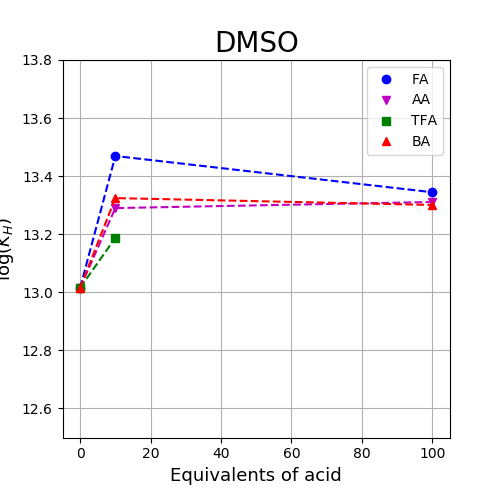
\includegraphics[width=\textwidth]{n2phys/dmso-henry}%
        \caption{}%
        \label{def:fgr:n2phys-dmso-henry}
    \end{subfigure}%

    \begin{subfigure}{0.25\linewidth}
        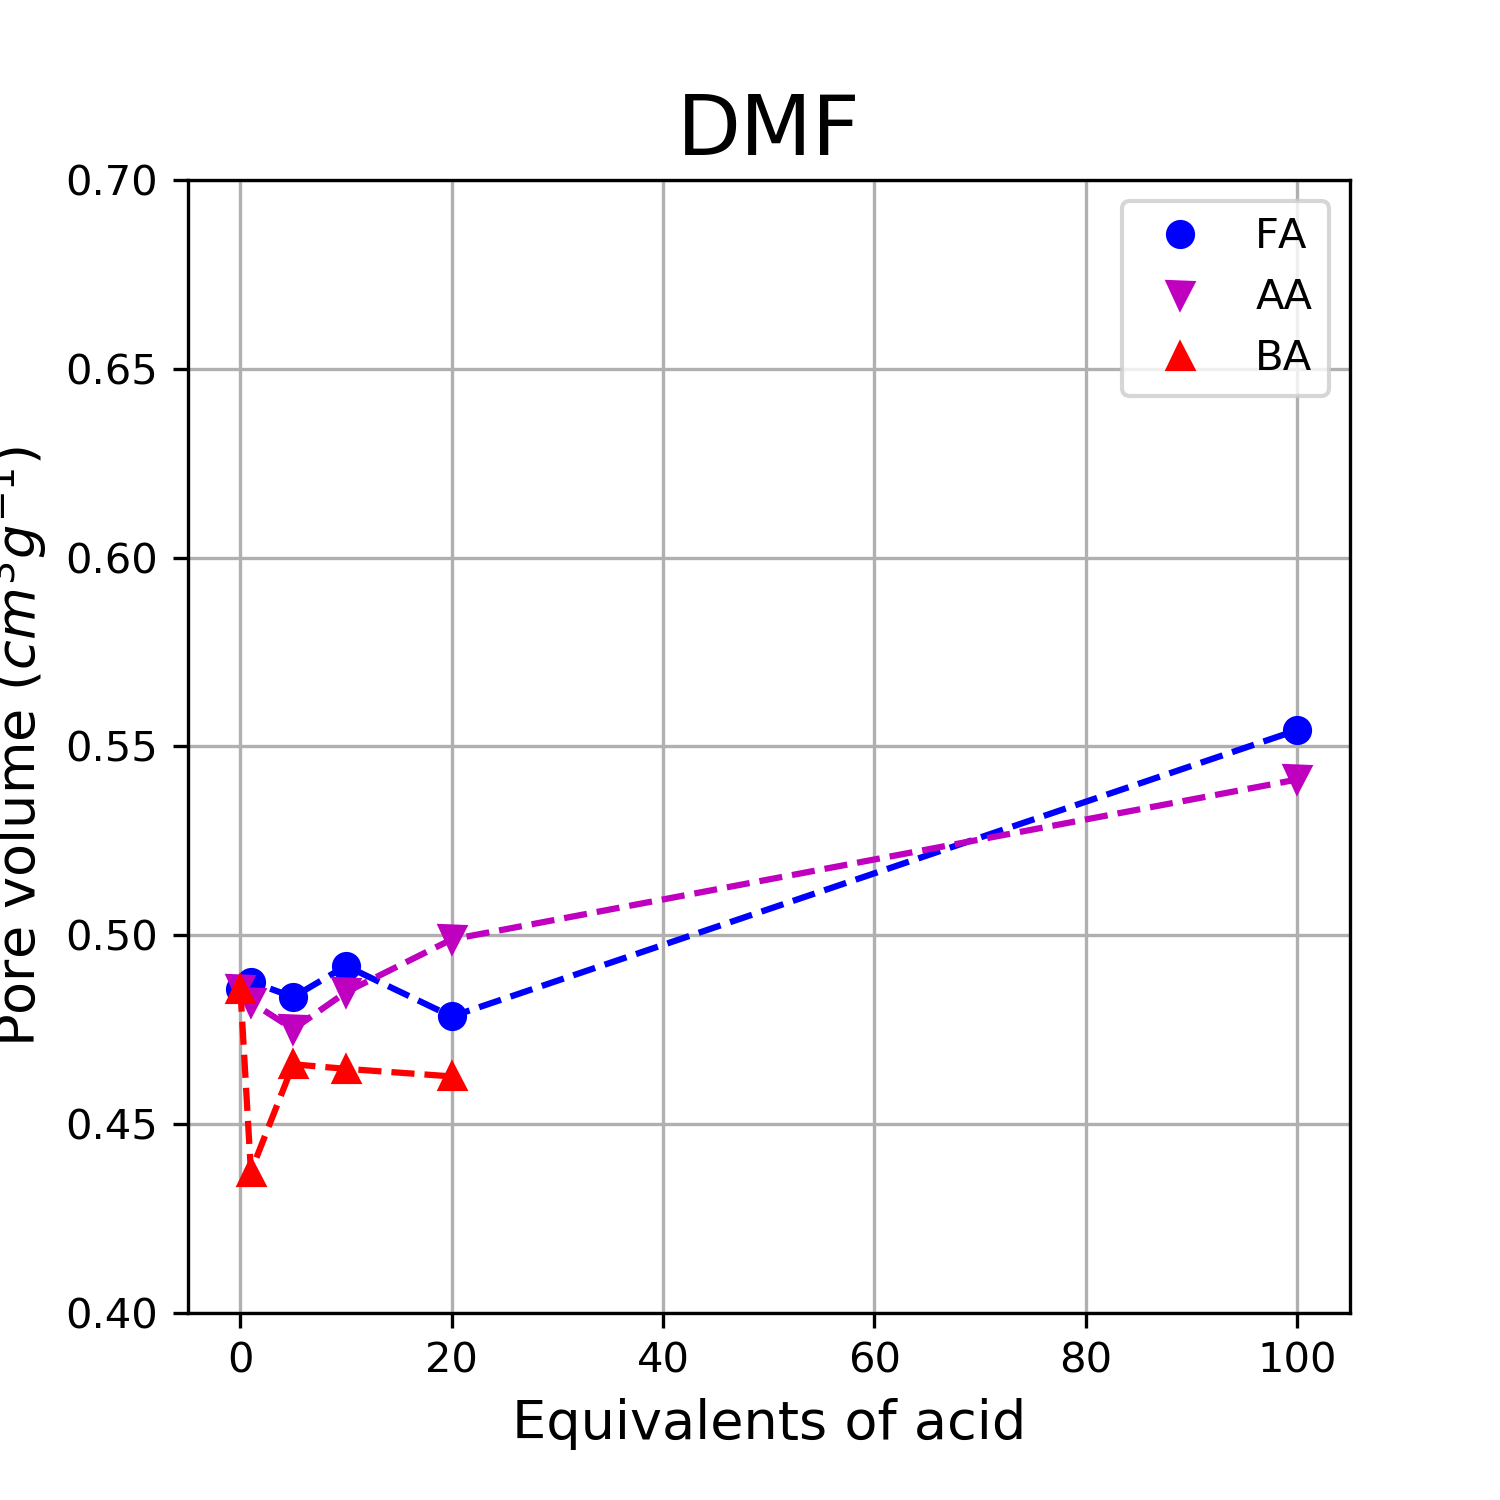
\includegraphics[width=\textwidth]{n2phys/dmf-porevol}%
        \caption{}%
        \label{def:fgr:n2phys-dmf-porevol}
    \end{subfigure}%
    \begin{subfigure}{0.25\linewidth}
        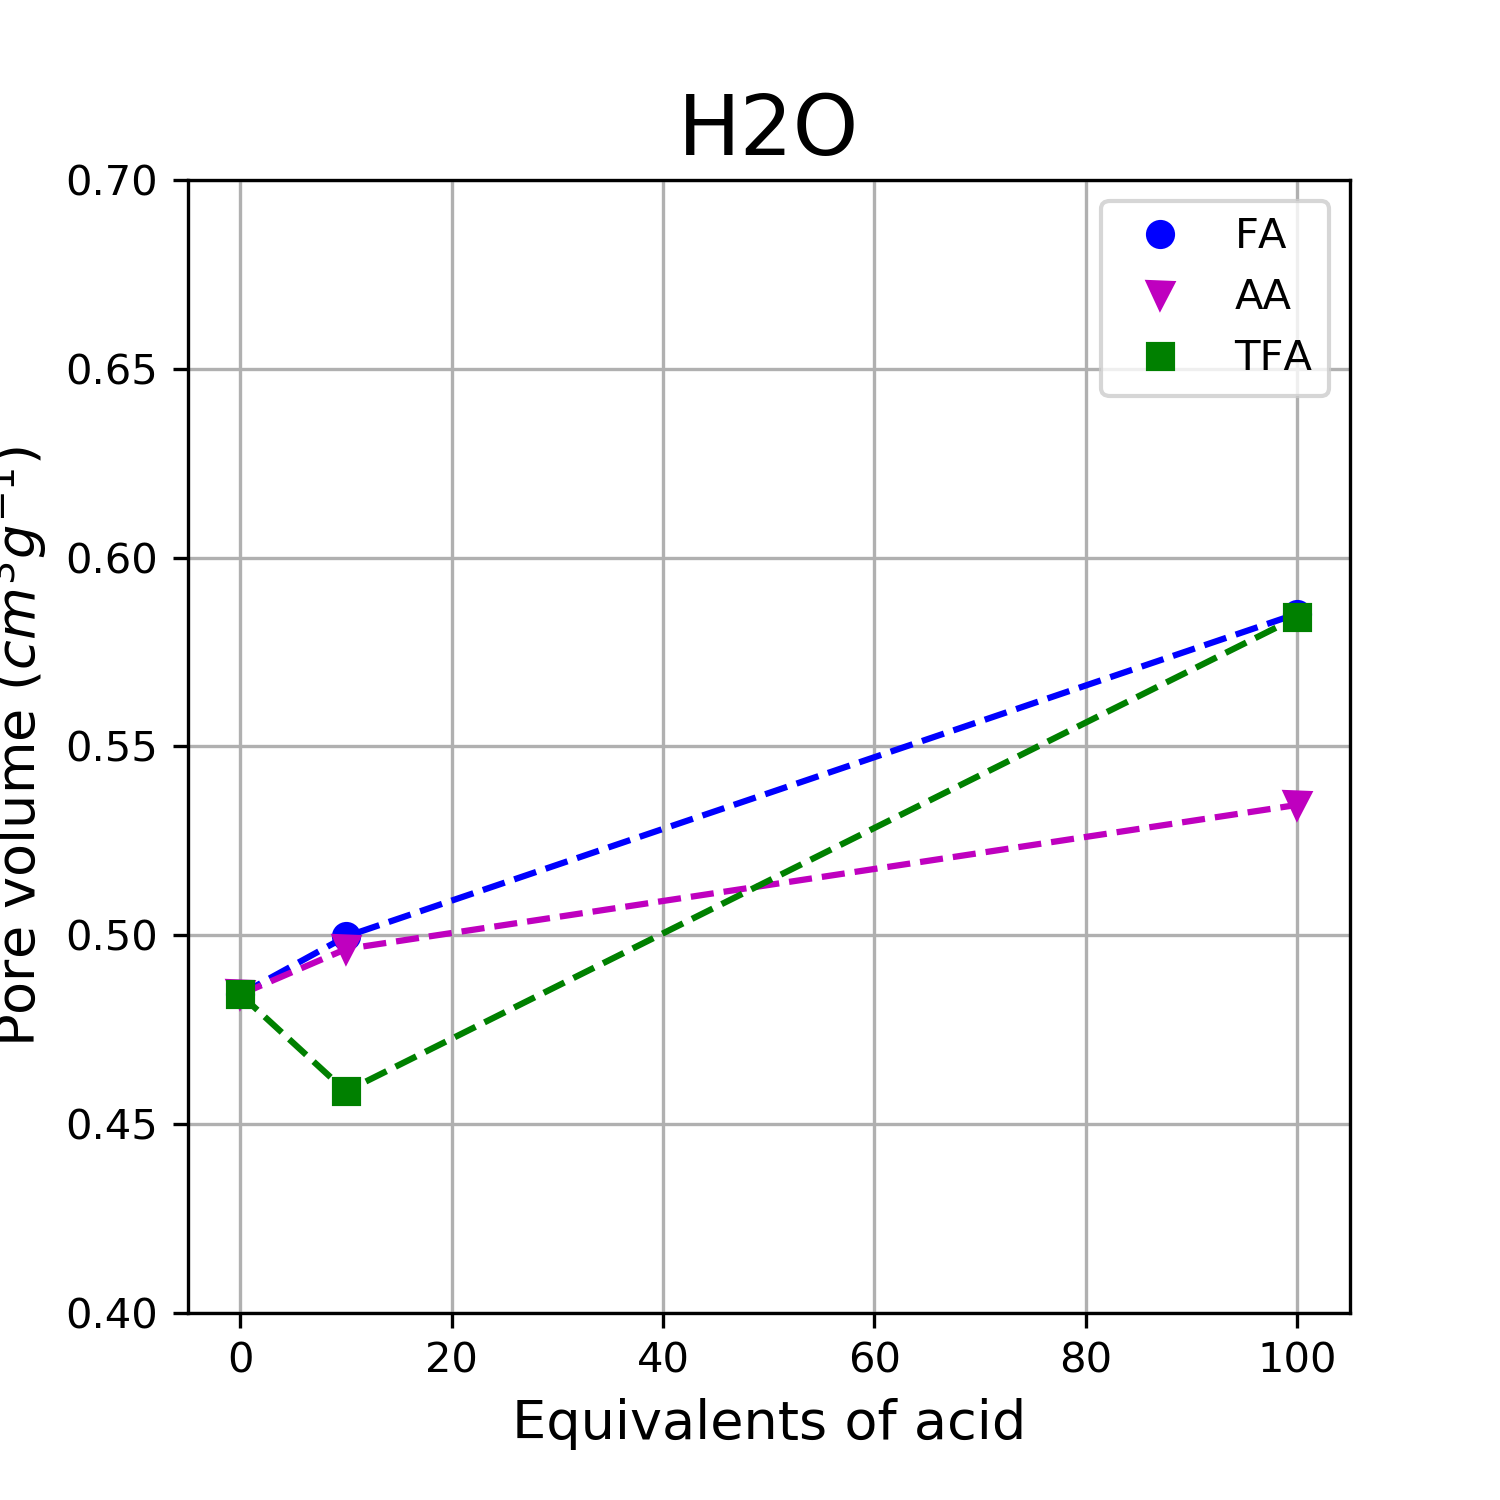
\includegraphics[width=\textwidth]{n2phys/h2o-porevol}%
        \caption{}%
        \label{def:fgr:n2phys-h2o-porevol}
    \end{subfigure}%
    \begin{subfigure}{0.25\linewidth}
        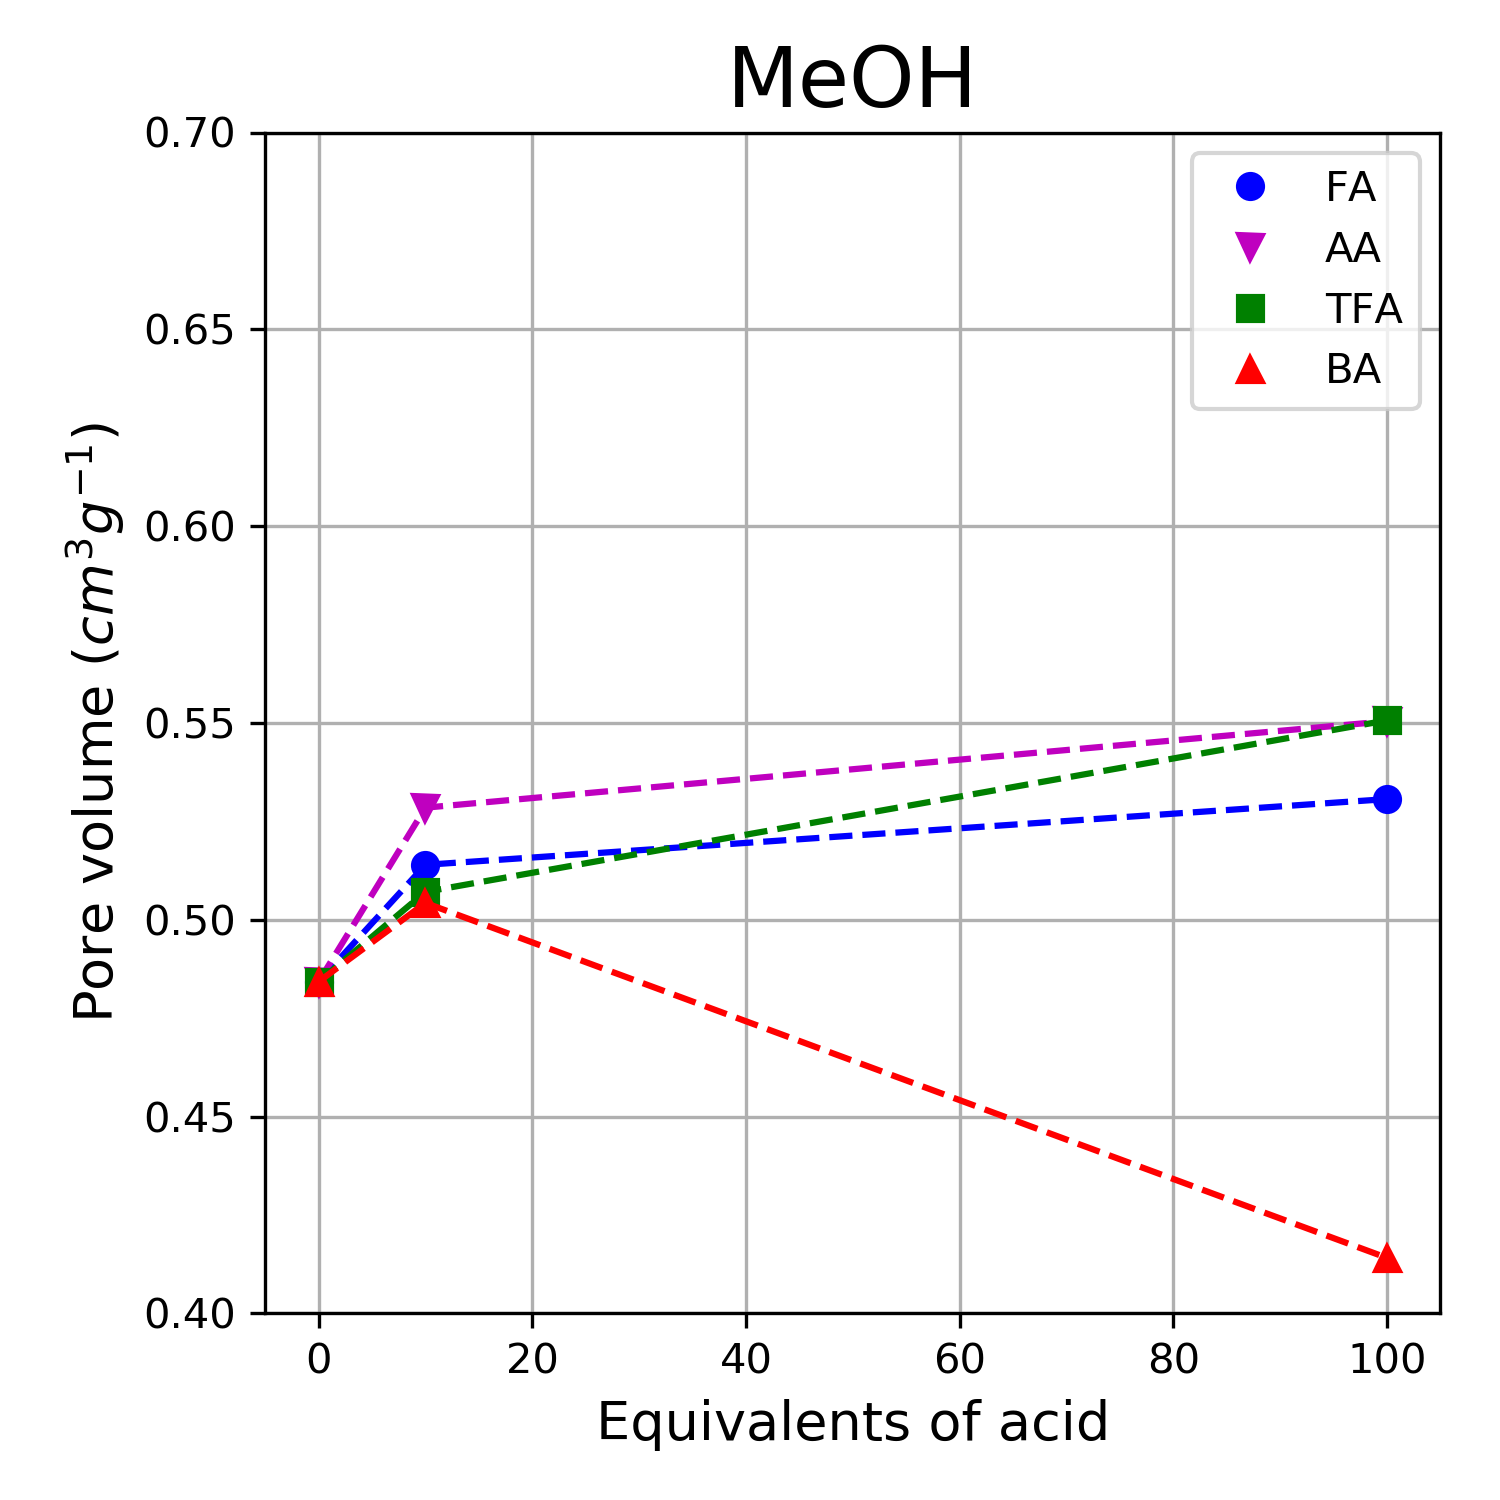
\includegraphics[width=\textwidth]{n2phys/meoh-porevol}%
        \caption{}%
        \label{def:fgr:n2phys-meoh-porevol}
    \end{subfigure}%
    \begin{subfigure}{0.25\linewidth}
        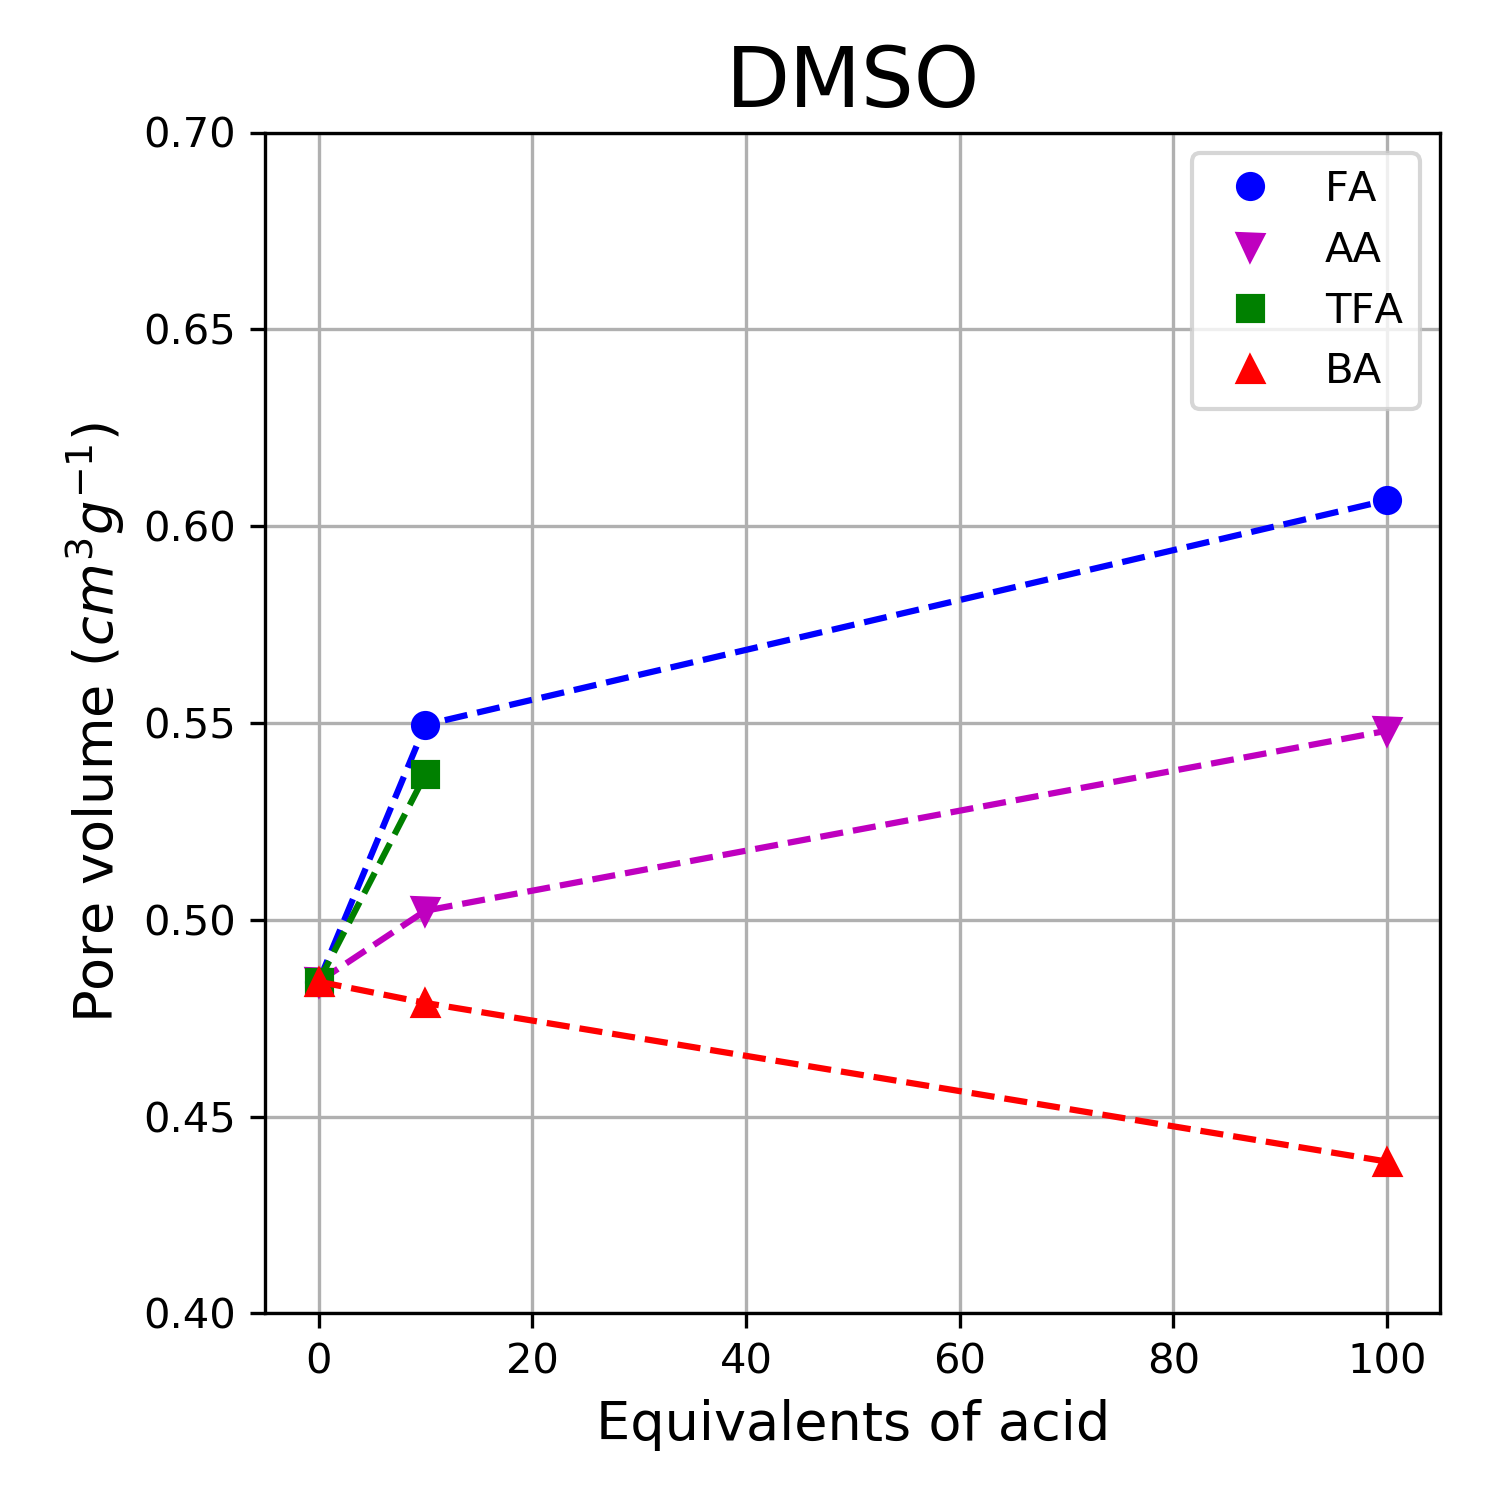
\includegraphics[width=\textwidth]{n2phys/dmso-porevol}%
        \caption{}%
        \label{def:fgr:n2phys-dmso-porevol}
    \end{subfigure}%

    \caption{Characterisation of all samples through predictors
    obtained through processing of the nitrogen physisorption 
    data at \SI{200}{\degreeCelsius}. The figure shows BET surface
    area (a-d), the logarithm of the initial Henry constant (e-h), 
    and calculated pore volume (i-l) for DMF, \ce{H2O}, MeOH and 
    DMSO leached materials, respectively.}%
    \label{def:fgr:nitrogen-predictors}
    
\end{figure}

The influence of the acid on the linker-to-node ratio appears to be
constant throughout the solvents used, with an overall trend of 
TFA > FA > AA > BA. The order is similar
to the acidic character of the compounds, except for
benzoic acid which has a lower pKa (4.2) than acetic acid (4.7).
The result is in accordance to the trend published by 
\citeauthor{shearerDefectEngineeringTuning2016} when analysing
the influence of these acids as used during modulated synthesis on the
defectivity of the resulting material~\cite{shearerDefectEngineeringTuning2016}.

When examining the influence of the solvent, another trend appears
to emerge, with samples leached in DMSO having the largest propensity
for defect generation, followed by DMF, water and methanol. In fact,
a sample with high concentration of TFA cannot be obtained, as the 
framework simply dissolves in the solution.
The contribution of the of the solvent is not as easy to determine due
to the complex interplay of multiple factors.
The polarity of the solvent molecule has been linked to 
the speed of post synthetic ligand exchange from
pristine UiO-66(Zr)~\cite{kimPostsyntheticLigandExchange2012}. The leaching
results do not, however, conform to the same trend, as water with a 
relative polarity of 1.0 introduces more defects than methanol 
(0.7) while DMF (0.38) is less effective than 
DMSO (0.44). The solubility of terephtalic acid in the solvent 
of choice may likely be a limiting factor driving its removal
from the framework. Water, which has the lowest solubility for 
BTC, is one of the better solvents for defect generation, likely
due to the high temperature of the reaction. As a strong acid
is added, the equilibrium shifts even more towards the 
left, which may explain the worse performance of low equivalents of TFA
in water as seen from adsorption predictors. At high concentrations,
it is likely that the rate constant for the protonation of the 
metal-oxygen bond starts to dominate the leaching process.
The viscosity of the 
solvent may also play a role in the mass transport of compounds 
through the porous media. However, the liquid with the highest 
kinematic viscosity, DMSO is actually the top performer during leaching,
indicating that mass transfer is not a factor.


\begin{figure}[!h]
    \centering

    \begin{subfigure}{0.25\linewidth}
        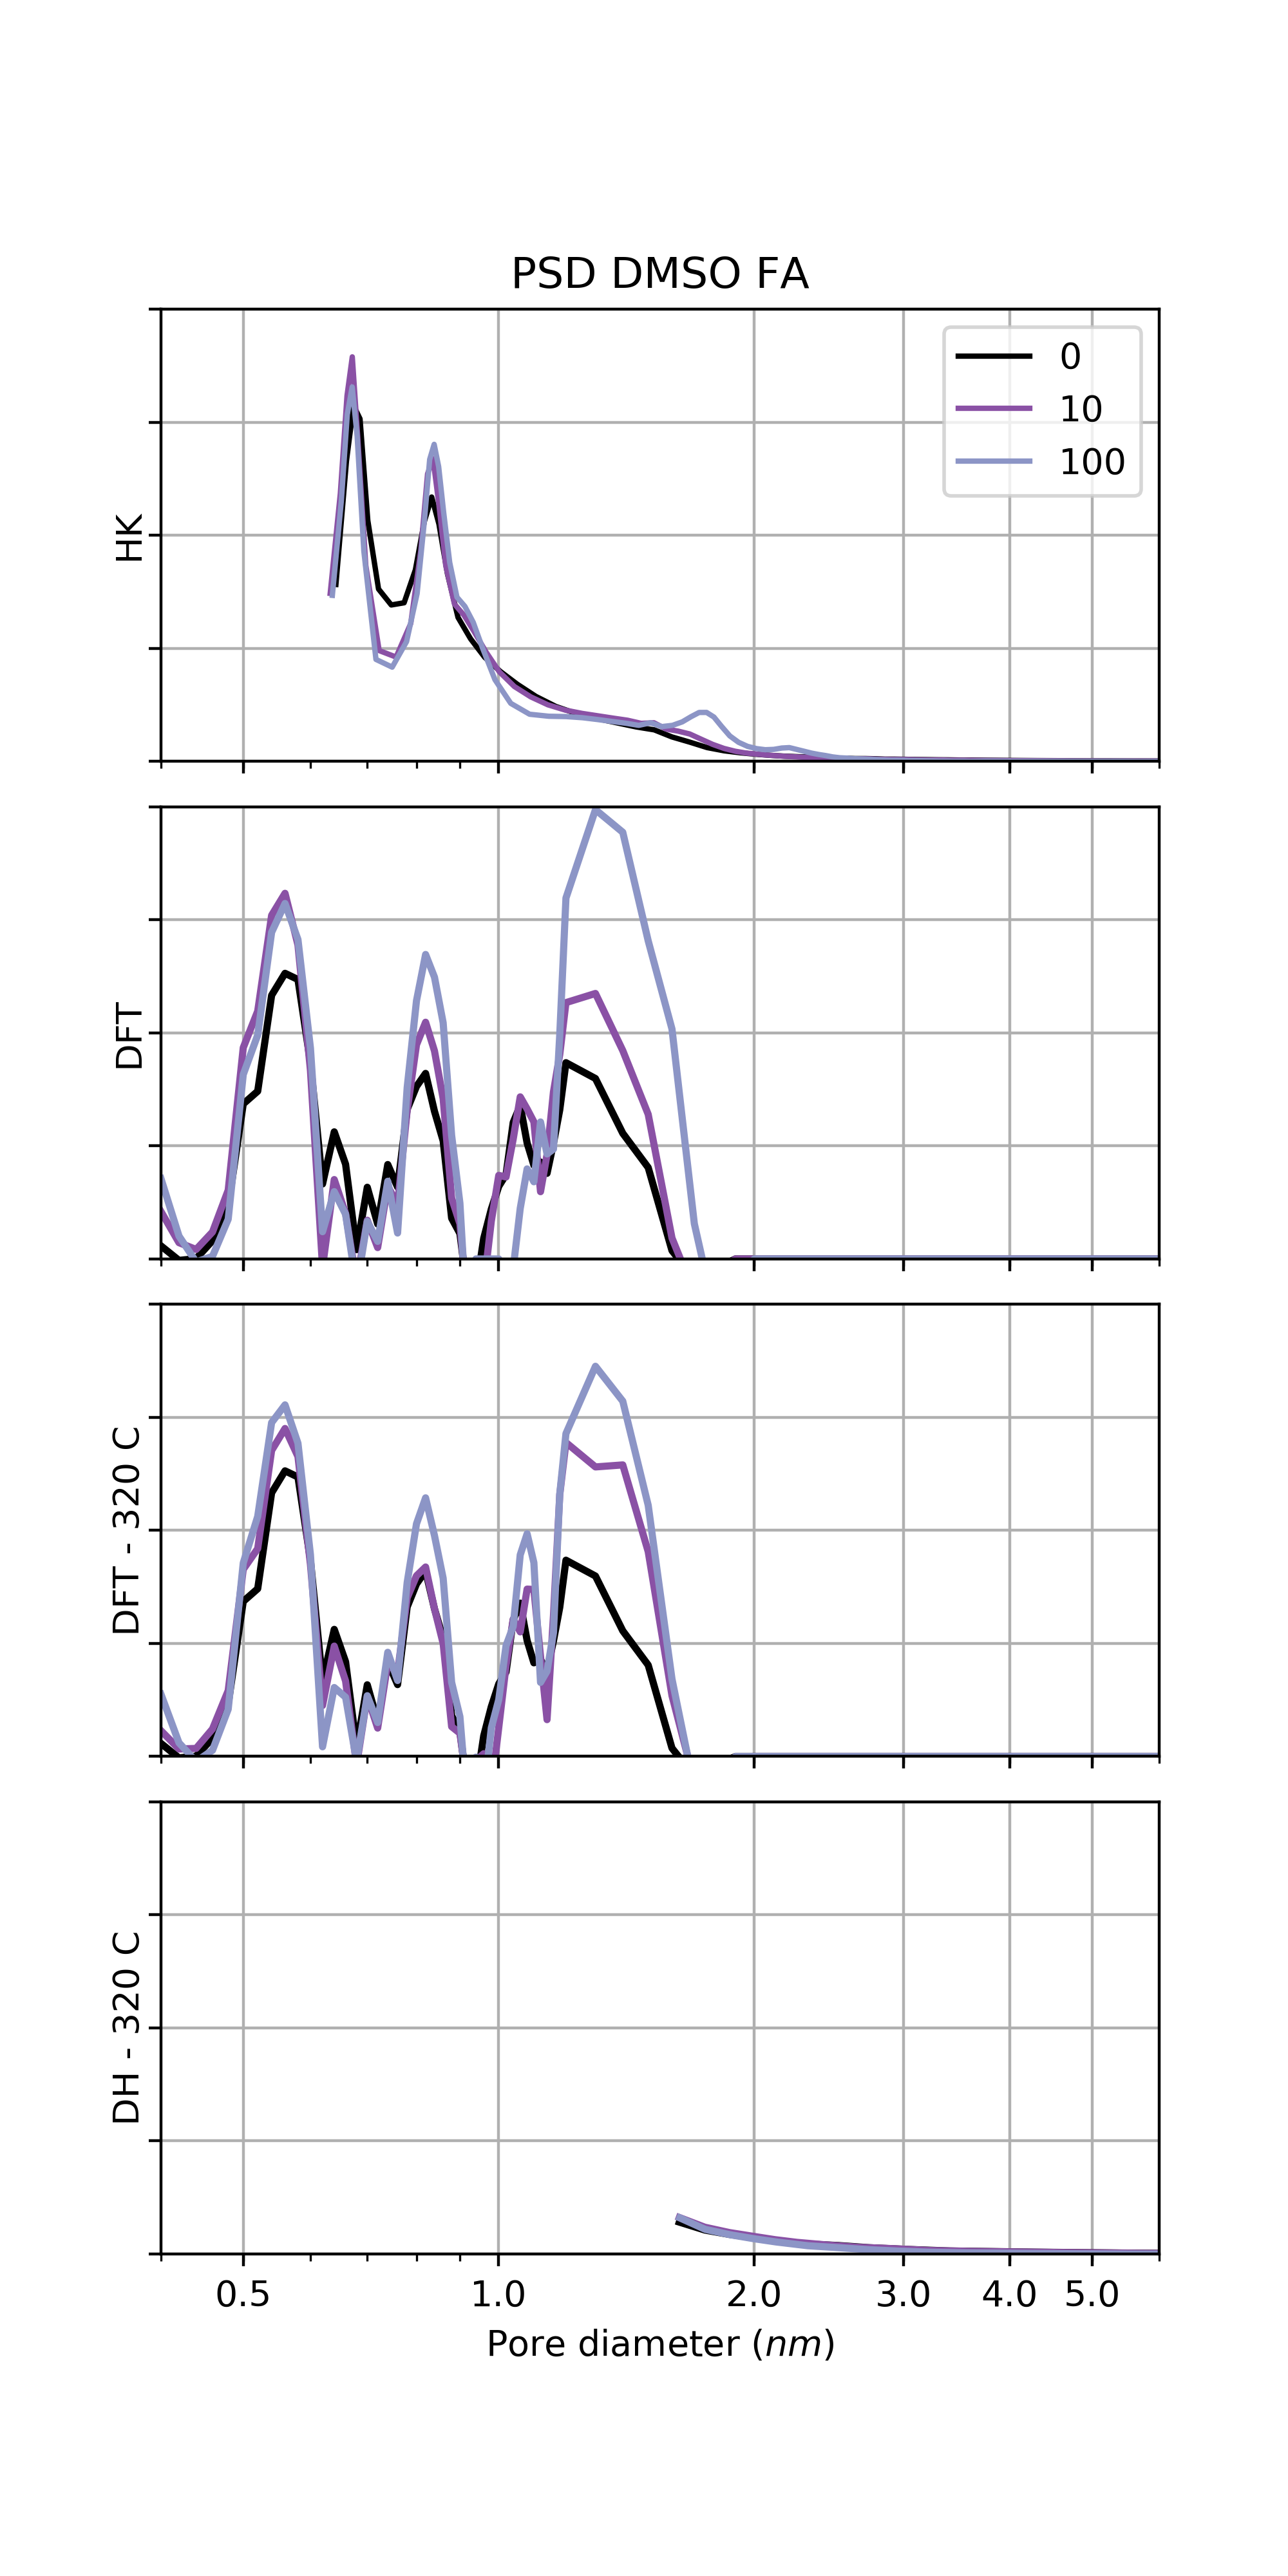
\includegraphics[width=\textwidth]{n2phys/dmso-fa-psd-complete}%
        \caption{}%
        \label{def:fgr:psd-dmso-fa}
    \end{subfigure}%
    \begin{subfigure}{0.25\linewidth}
        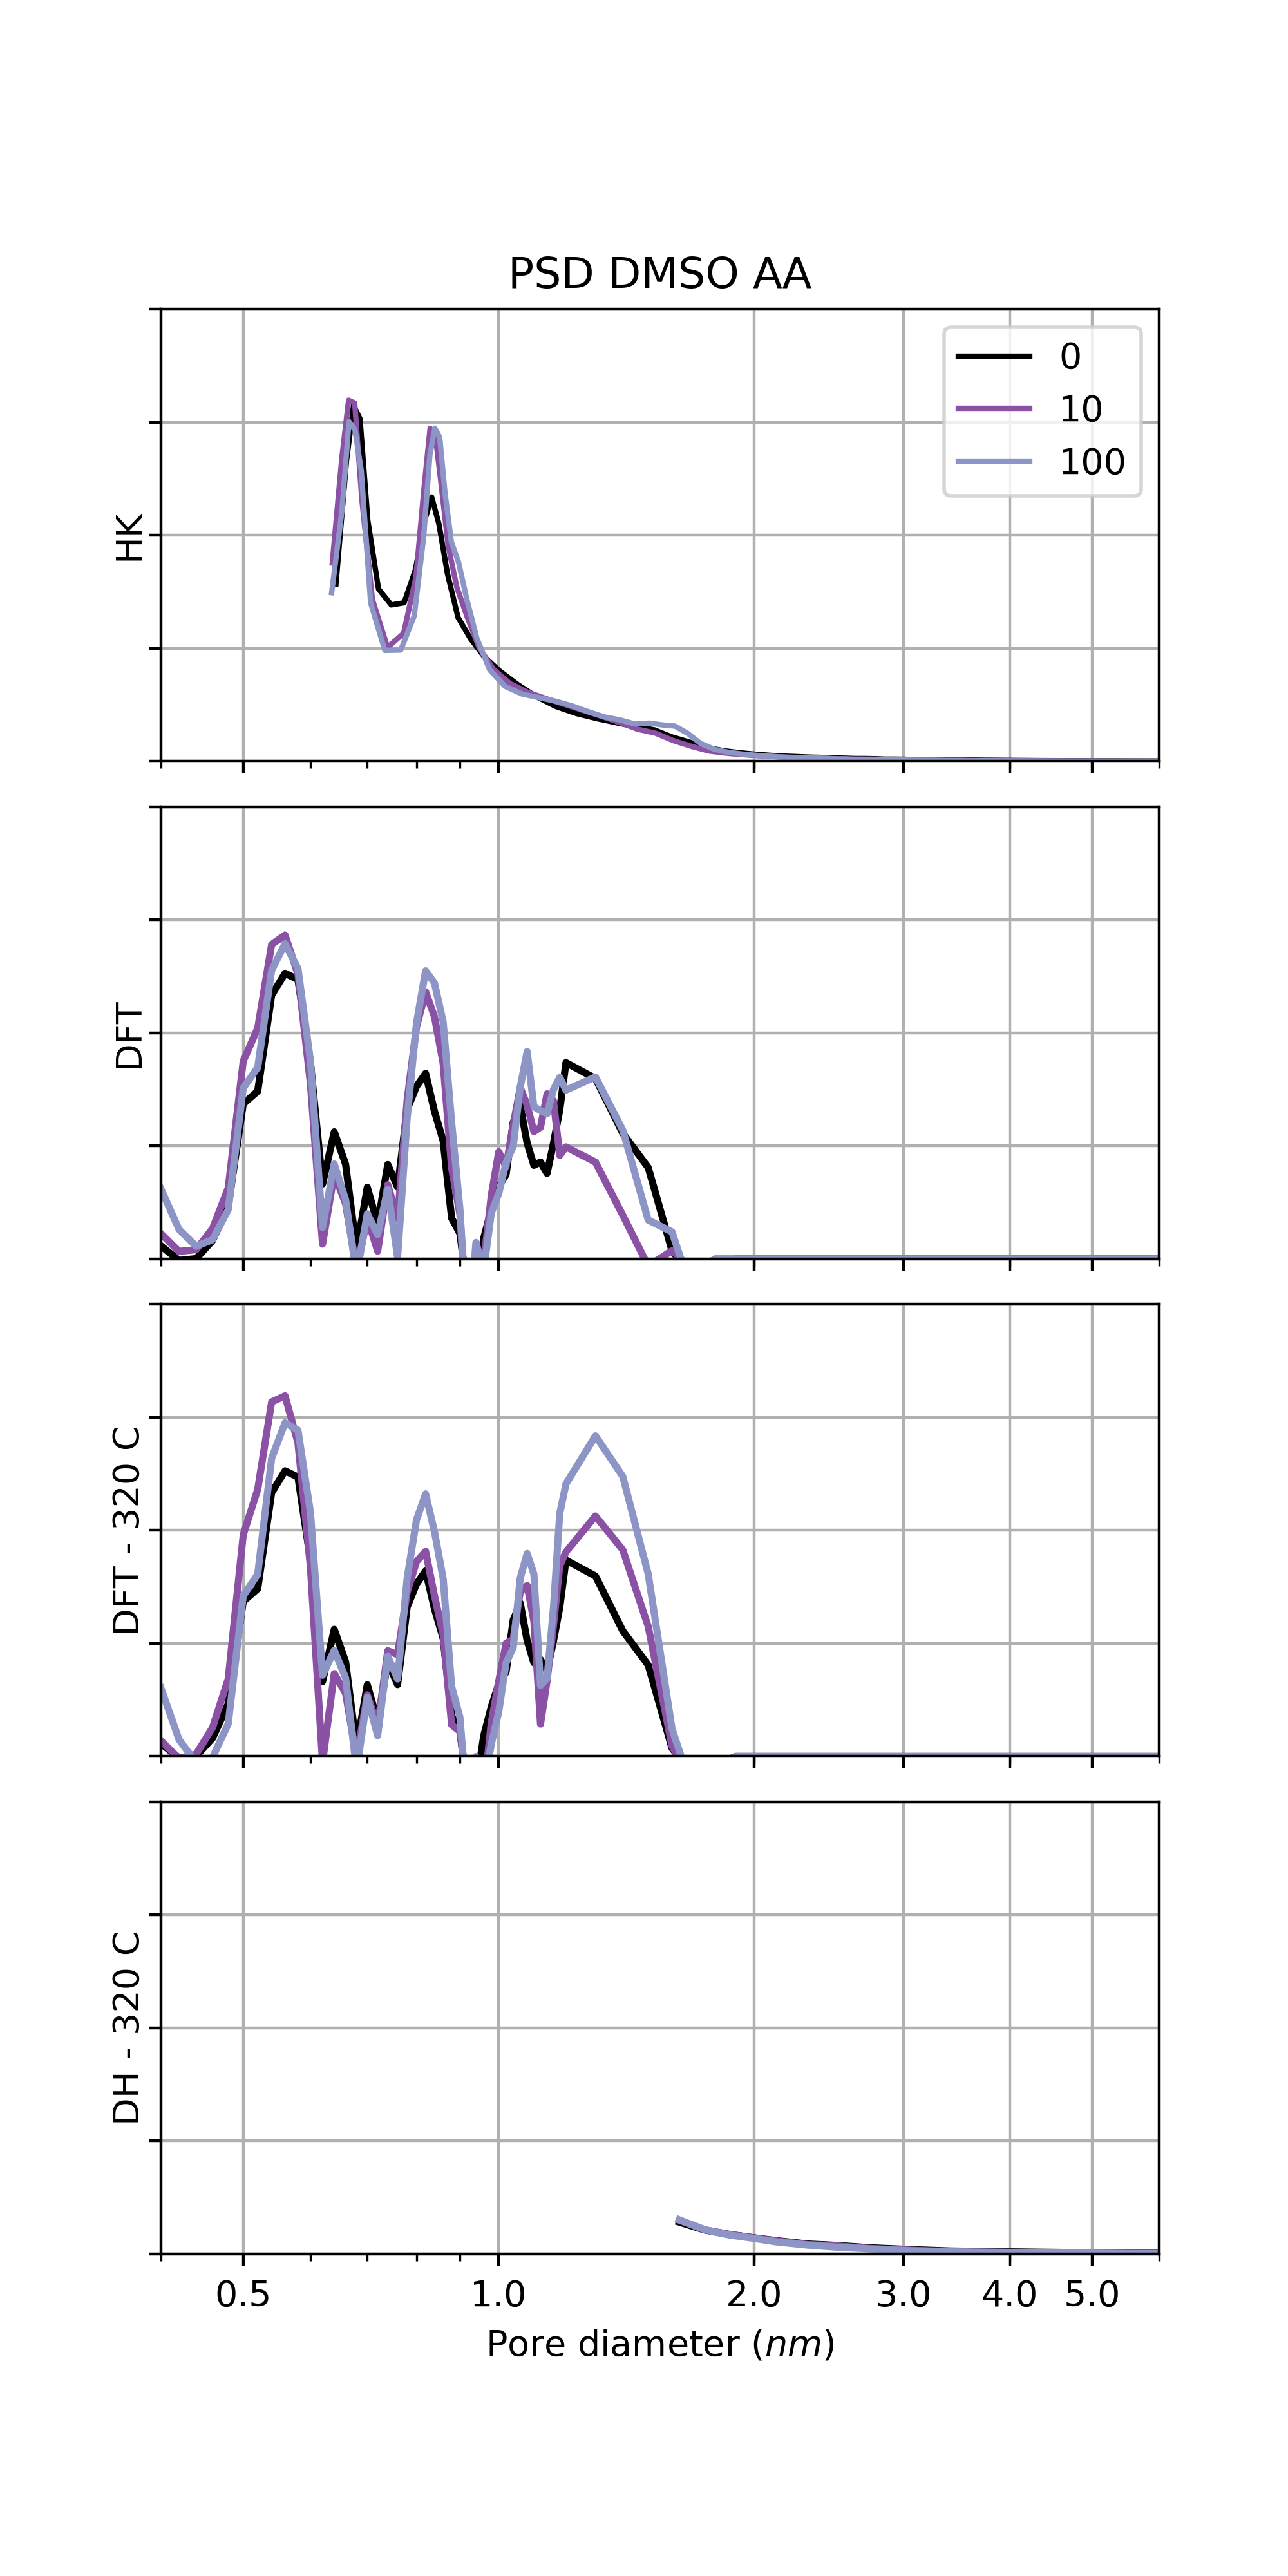
\includegraphics[width=\textwidth]{n2phys/dmso-aa-psd-complete}%
        \caption{}%
        \label{def:fgr:psd-dmso-aa}
    \end{subfigure}%
    \begin{subfigure}{0.25\linewidth}
        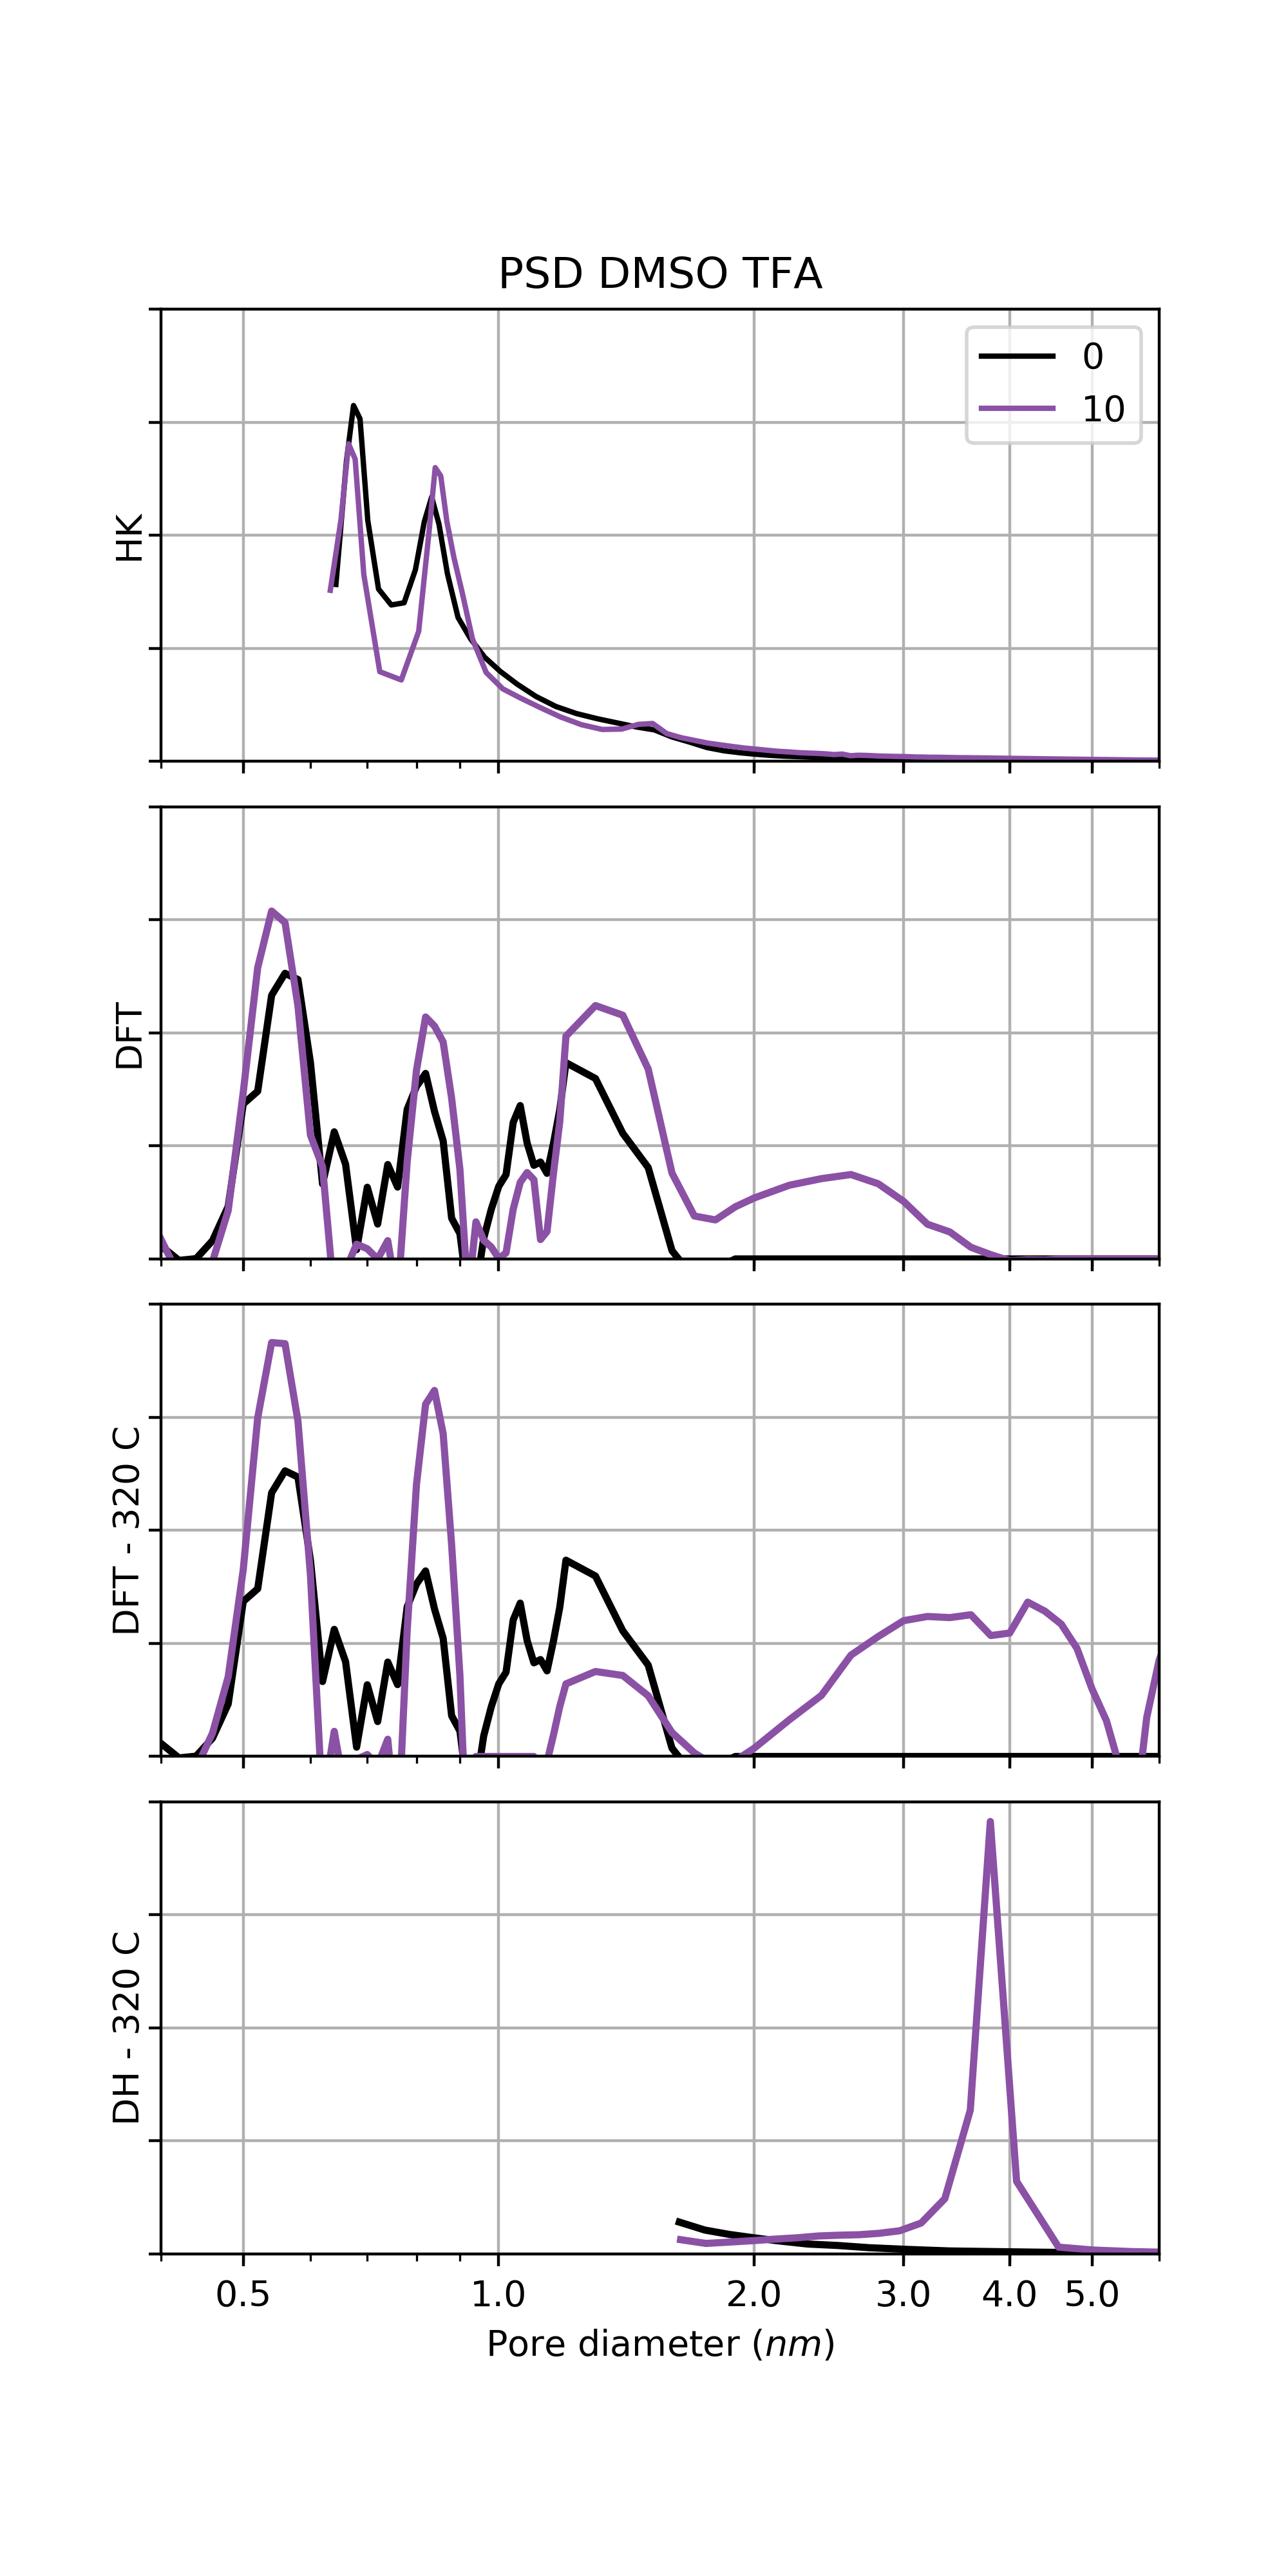
\includegraphics[width=\textwidth]{n2phys/dmso-tfa-psd-complete}%
        \caption{}%
        \label{def:fgr:psd-dmso-tfa}
    \end{subfigure}%
    \begin{subfigure}{0.25\linewidth}
        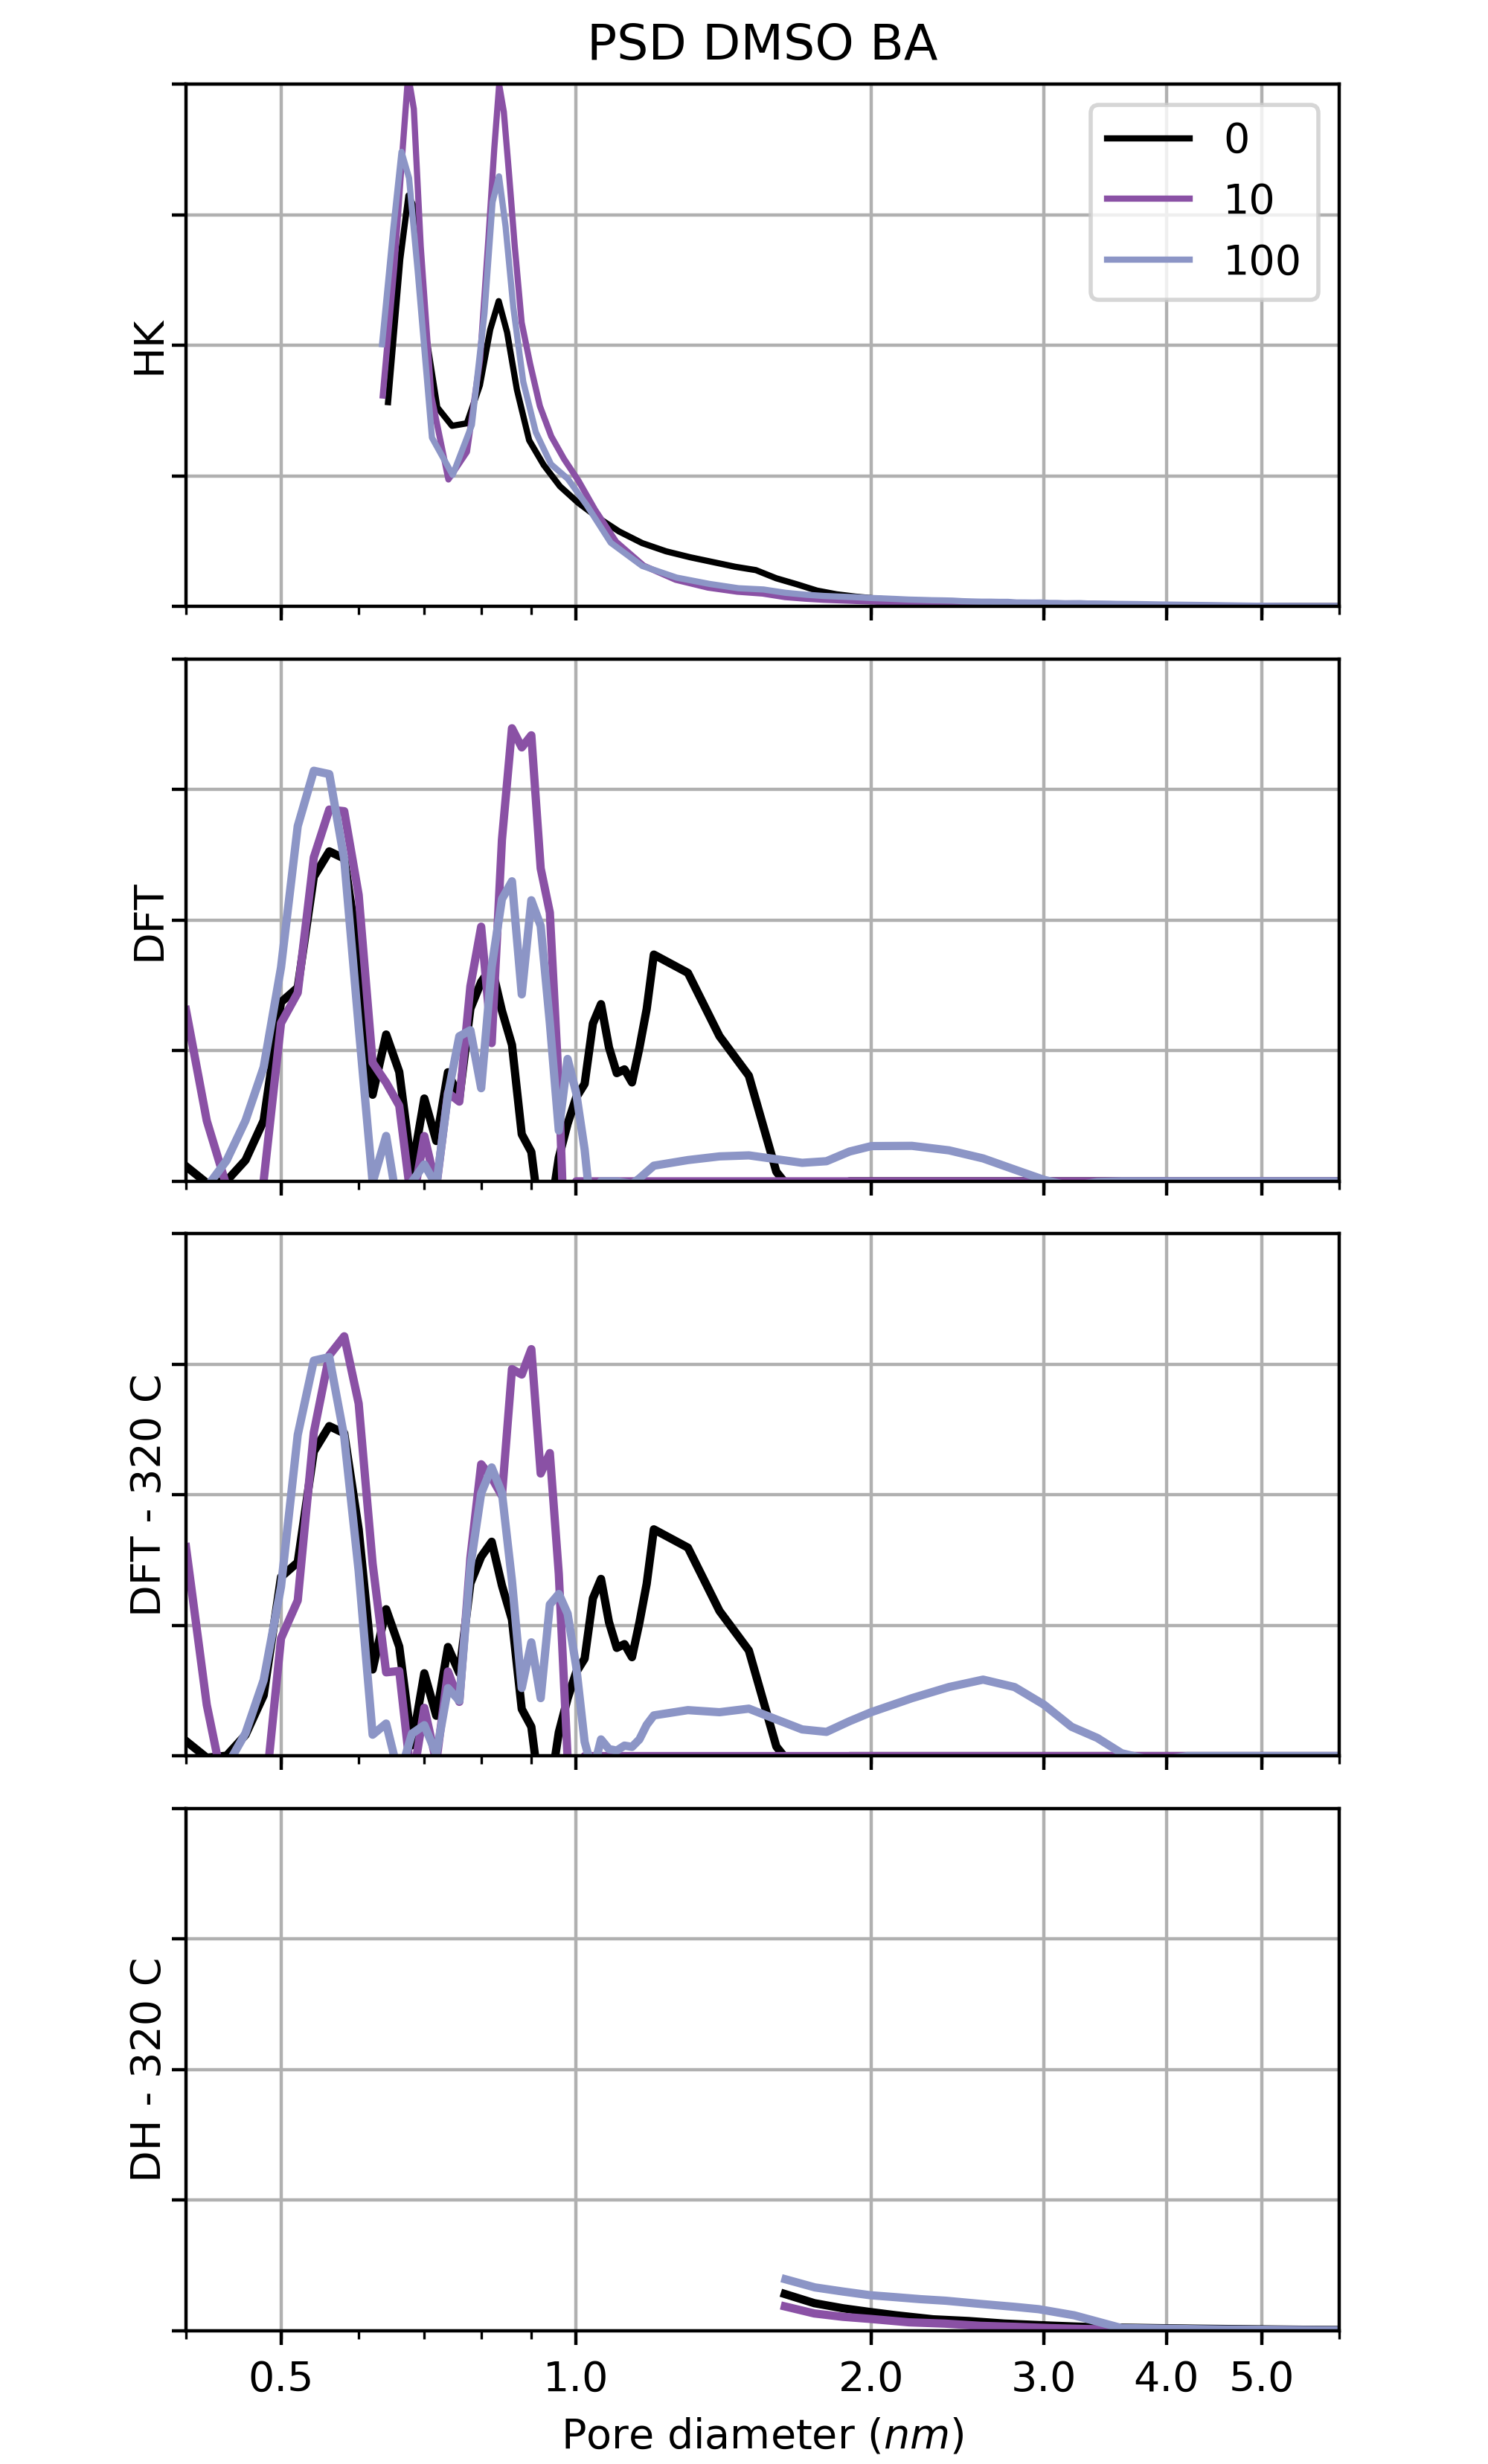
\includegraphics[width=\textwidth]{n2phys/dmso-ba-psd-complete}%
        \caption{}%
        \label{def:fgr:psd-dmso-ba}
    \end{subfigure}%

    \caption{Pore size distribution for the DMSO-leached
    samples as resulting from the HK (top), DFT (middle) and DH 
    (bottom) methods on (a) formic acid, (b) acetic acid, (c) TFA and 
    (d) BA. The top and bottom two distributions are
    calculated on the low and high temperature activated material
    respectively. The parent material is depicted in black.}%
    \label{def:fgr:psd}
        
\end{figure}

The calculated pore sizes with both the HK method and the DFT method 
show two sharp peaks corresponding to the octahedral and tetrahedral
pores in the UiO-66 structure. In \autoref{def:fgr:psd}, the pore
size distribution for the DMSO dataset is depicted, for both low
temperature and high temperature activated variants. The appearance of 
a tertiary pore is visible in the leached samples with formic,
acetic and trifluoroacetic acid. This pore size likely corresponds
to the increased pore volume introduced by missing linker-type 
defects. The calculated diameter of this tertiary pore is
inversely proportional to the molecular size of the 
leaching compound used, which is a clear indication of the presence of 
the acid molecules in the structure as capping agents. On the samples
which have been activated at \SI{320}{\degreeCelsius}, the pore width
shifts to a single value as the coordinated acids are evacuated.

The pore size distribution calculated in the benzoic acid leached
samples shows the disappearance of peaks larger than around 
\SI{1}{\nano\metre}, as the compound replaces formate as the 
capping agent for the initial defects in the structure. Due to the 
similarity of the terephtalate linker with benzoate, the structure
becomes more ``ideal'' than the pristine material. At high concentrations
of benzoic acid, an overall decrease in porosity may be seen, as 
two benzoate molecules may act as capping agents in adjacent 
sites (\autoref{def:fgr:benzoic-defect}), effectively 
lowering the available pore volume. The effect is corroborated 
by trends in the linker-to-node ratio, surface area and total 
pore volume in both methanol, DMSO and to a lesser extent DMF.

\begin{wrapfigure}[15]{r}{0.3\textwidth}
    \centering
    \captionsetup{format=plain}
    \fbox{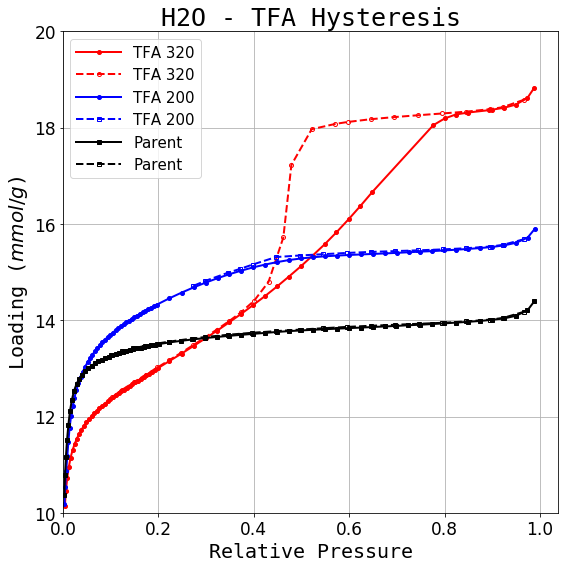
\includegraphics[width=0.28\textwidth]{n2phys/dmso-tfa-hysteresis}}
    \caption{Hysteresis loop in high temperature activated TFA treated 
    UiO-66(Zr)}%
    \label{def:fgr:ht-hysteresis}
\end{wrapfigure}

At very high concentrations of TFA and BA, a fourth pore size
begins to be appear in the DFT calculated pore distribution.
This is likely evidence that missing cluster defects can be 
introduced at these concentrations. It should be noted that 
if such large-scale modifications of the structure are possible,
complete structural breakdown is not far away. Indeed, samples with 
higher concentrations of acid could not be obtained with TFA in DMSO,
with sample subjected to these conditions ending up completely
dissolved. The appearance of this type of porosity in the samples
treated with benzoic acid is counterintuitive, as the TGA linker
ratio does not allude to any changes in coordination. In this case,
it could be that missing cluster defects are still generated
forming a \textbf{reo}-benz phase~\cite{atzoriEffectBenzoicAcid2017} 
while the excess of ``dangling'' benzoate moieties in the framework 
account for the decrease in surface area and capacity.

No hysteresis curve is observable on any samples activated at 
\SI{200}{\degreeCelsius}. When activating at higher temperature,
a hysteresis curve appears in the high concentration leached
TFA samples (\autoref{def:fgr:ht-hysteresis}), which corresponds to
a pore size of around \SI{4}{\nano\metre} in both DFT and DH calculated
pore distribution. The shape of the hysteresis loop is also 
reminiscent of condensation in ink bottle-like pores, suggesting
the existence of voids within the crystal matrix which are 
not directly accessible. This further confirms how effective 
highly acidic solutions can be at defect generation.